\documentclass[12pt, letterpaper]{report}

% =========================================================
% FORMATO PUCV
% =========================================================

\usepackage{pucv_inf_2024}
\usepackage{tikz}

% Idioma: partición silábica en español.
% Solo se activa si la distribución de LaTeX tiene instalado el idioma
% (paquete 'texlive-langspanish' o equivalente). Sin él, el documento
% compila igual, pero la separación silábica usa las reglas del inglés.
% 'es-noshorthands' evita que babel active caracteres (", <, >, ', ~)
% que interferirían con el resto de los paquetes.
\IfFileExists{spanish.ldf}{%
    \usepackage[spanish, es-tabla, es-noshorthands]{babel}%
}{}

% =========================================================
% PAQUETES ADICIONALES
% =========================================================

\usepackage{graphicx}
\usepackage{float}
\usepackage{booktabs}
\usepackage{tabularx}
\usepackage{array}
\usepackage{longtable}
\usepackage{multirow}
\usepackage{colortbl}
\usepackage{pdflscape}
\usepackage[most]{tcolorbox}
\usepackage[hidelinks]{hyperref}

% Carpeta donde se encuentran los gráficos
\graphicspath{{Figuras/}{Figuras/diagramas/}}

% =========================================================
% ESTILOS PROPIOS DEL INFORME
% =========================================================

% =========================================================
% ESTILOS Y COMANDOS PROPIOS DEL INFORME
% Complementa a pucv_inf_2024.sty sin modificarlo.
% =========================================================

% ---------------------------------------------------------
% Rótulos en español
% Se reaplican después de babel para conservar los títulos de
% índices definidos por pucv_inf_2024.sty.
% ---------------------------------------------------------

\AtBeginDocument{%
    \renewcommand{\figurename}{Figura}%
    \renewcommand{\tablename}{Tabla}%
    \renewcommand{\nomname}{\uppercase{Lista de Símbolos}}%
    \renewcommand{\contentsname}{\uppercase{Índice General}}%
    \renewcommand{\listfigurename}{\uppercase{Lista de Figuras}}%
    \renewcommand{\listtablename}{\uppercase{Lista de Tablas}}%
    \renewcommand{\chaptername}{Capítulo}%
    \renewcommand{\appendixname}{Anexo}%
}

% ---------------------------------------------------------
% Bibliografía en español
% Fuerza los rótulos APA en español («Recuperado el ... de»,
% «2.ª ed.», «y» en lugar de «and») sin depender de babel.
% ---------------------------------------------------------

\ExecuteBibliographyOptions{language = spanish}
\DeclareLanguageMapping{spanish}{spanish-apa}

% ---------------------------------------------------------
% Colores auxiliares
% ---------------------------------------------------------

\definecolor{notacolor}{HTML}{4472c4}   % azul institucional (igual a titlecolor)
\definecolor{notafondo}{HTML}{EEF2FA}
\definecolor{pendientecolor}{HTML}{B85C00}
\definecolor{pendientefondo}{HTML}{FDF3E7}
\definecolor{filacabecera}{HTML}{DCE6F5}

% ---------------------------------------------------------
% Cajas de nota y de tareas pendientes
% (equivalen a las citas en bloque y a los bloques
%  "POR COMPLETAR" del documento original en Markdown)
% ---------------------------------------------------------

\newtcolorbox{nota}[1][]{%
    enhanced,
    breakable,
    colback = notafondo,
    colframe = notacolor,
    boxrule = 0pt,
    leftrule = 3pt,
    arc = 0pt,
    outer arc = 0pt,
    left = 8pt, right = 8pt, top = 6pt, bottom = 6pt,
    fontupper = \small,
    parbox = false,
    #1
}

\newtcolorbox{pendiente}[1][Por completar]{%
    enhanced,
    breakable,
    colback = pendientefondo,
    colframe = pendientecolor,
    boxrule = 0.6pt,
    arc = 2pt,
    left = 8pt, right = 8pt, top = 6pt, bottom = 6pt,
    fontupper = \small,
    parbox = false,
    title = {\footnotesize\bfseries\MakeUppercase{#1}},
    coltitle = white,
    colbacktitle = pendientecolor
}

% Marca breve, para usar dentro de una línea de texto
\newcommand{\porcompletarinline}[1]{%
    \textcolor{pendientecolor}{\textbf{[por completar: #1]}}%
}

% ---------------------------------------------------------
% Estilo común de las tablas largas
% ---------------------------------------------------------

\newcommand{\estilotabla}{%
    \footnotesize
    \setlength{\parskip}{0pt}%
    \setlength{\parindent}{0pt}%
    \setlength{\tabcolsep}{4pt}%
    \renewcommand{\arraystretch}{1.25}%
}

\newcommand{\estilotablachica}{%
    \estilotabla
    \scriptsize
}

% Separación antes y después de las longtable
\setlength{\LTpre}{8pt}
\setlength{\LTpost}{8pt}

% Columnas de párrafo centradas verticalmente arriba
\newcolumntype{L}[1]{>{\raggedright\arraybackslash}p{#1}}
\newcolumntype{C}[1]{>{\centering\arraybackslash}p{#1}}

% ---------------------------------------------------------
% Identificadores de código, clases y estados
% ---------------------------------------------------------

\newcommand{\clase}[1]{\texttt{#1}}
\newcommand{\estado}[1]{\texttt{#1}}
\newcommand{\este}[1]{\textit{#1}}

% Estereotipos UML
\newcommand{\ster}[1]{\texttt{\guillemotleft #1\guillemotright}}

% ---------------------------------------------------------
% Figuras de diagramas: comando abreviado
% #1 ancho relativo · #2 archivo · #3 título breve (Lista de Figuras)
% #4 leyenda completa · #5 etiqueta
% ---------------------------------------------------------

\newcommand{\figuradiagrama}[5]{%
    \begin{figure}[H]
        \centering
        \includegraphics[width=#1\textwidth]{#2}
        \caption[#3]{#4}
        \label{#5}
    \end{figure}%
}

% ---------------------------------------------------------
% Formato de los anexos: "Anexo A." en lugar de "A."
% ---------------------------------------------------------

\newcommand{\formatoanexos}{%
    \renewcommand{\thechapter}{Anexo~\Alph{chapter}}%
    \setcounter{figure}{0}%
    \setcounter{table}{0}%
}

% ---------------------------------------------------------
% Ajustes de listas y espaciado dentro de entornos
% ---------------------------------------------------------

\setlist[itemize]{leftmargin=1.2cm, itemsep=2pt, topsep=4pt}
\setlist[enumerate]{leftmargin=1.2cm, itemsep=2pt, topsep=4pt}

% Evita que hyperref rompa las referencias de longtable
\hypersetup{
    bookmarksnumbered = true,
    pdftitle = {Informe 2 - Modelamiento UML del sistema BeeTracer},
    pdfsubject = {ICI-3242 Modelamiento de Software - PUCV}
}


% =========================================================
% DATOS DE PORTADA
% =========================================================
% >>> Editar aquí los datos de la portada <<<

\newcommand{\tituloInforme}{%
    Informe 2: Modelamiento UML del sistema BeeTracer}
\newcommand{\subtituloInforme}{%
    Trazabilidad y evidencia fotográfica del desconsolidado
    en terminales extraportuarios}
\newcommand{\asignaturaInforme}{ICI-3242 Modelamiento de Software}
\newcommand{\profesorInforme}{Broderick Crawford}
\newcommand{\paraleloInforme}{3}
\newcommand{\fechaInforme}{Septiembre 2026}

% =========================================================
% REFERENCIAS
% =========================================================

\addbibresource{referencias.bib}

% =========================================================
% DOCUMENTO
% =========================================================

\begin{document}

% =========================================================
% PORTADA
% =========================================================

\begin{titlepage}

\thispagestyle{empty}

% =========================================================
% ENCABEZADO INSTITUCIONAL
% =========================================================

\begin{tikzpicture}[remember picture,overlay]

    \node[
        anchor=north,
        inner sep=0pt
    ] at (current page.north)
    {
        
\includegraphics[
            width=\paperwidth
        ]{Figuras/encabezado_pucv.png}
    };

\end{tikzpicture}


% =========================================================
% TÍTULO DEL INFORME
% =========================================================

\vspace*{8.4cm}

\begin{center}

    \begin{minipage}{0.80\textwidth}

        \centering

        {\color{titlecolor}
        \fontsize{20}{25}\selectfont
        \bfseries
        \MakeUppercase{\tituloInforme}
        \par}

        \vspace{0.55cm}

        {\color{titlecolor}
        \fontsize{13}{17}\selectfont
        \itshape
        \subtituloInforme
        \par}

    \end{minipage}

\end{center}


% =========================================================
% INTEGRANTES
% =========================================================

\vfill

\begin{flushright}

    \begin{minipage}{0.50\textwidth}

        \raggedright

        {\color{titlecolor}
        \large\bfseries
        \textsc{Benjamín Contreras}\\[0.04cm]
        \textsc{Renato Espina}\\[0.04cm]
        \textsc{Joaquín Guarda}\\[0.04cm]
        \textsc{Ignacio Ruiz}\\[0.04cm]
        \textsc{Sergio Codoceo}
        \par}


        \vspace{0.6cm}


        {\color{titlecolor}
        \large\bfseries
        \textsc{\asignaturaInforme}
        \par}

        \vspace{0.30cm}

        {\color{titlecolor}
        \normalsize
        \textbf{Profesor:} \profesorInforme
        \par}

        \vspace{0.10cm}

        {\color{titlecolor}
        \normalsize
        \textbf{Paralelo:} \paraleloInforme
        \par}

        \vspace{0.45cm}

        {\color{titlecolor}
        \large\bfseries
        \fechaInforme
        \par}

    \end{minipage}

\end{flushright}

\vspace{1.0cm}

\end{titlepage}


% =========================================================
% ÍNDICES
% =========================================================

\pagenumbering{roman}

\clearpage
\addcontentsline{toc}{chapter}{Índice General}
\tableofcontents

\clearpage
\addcontentsline{toc}{chapter}{Lista de Figuras}
\listoffigures

\clearpage
\addcontentsline{toc}{chapter}{Lista de Tablas}
\listoftables

% =========================================================
% CONTENIDO PRINCIPAL
% =========================================================

\clearpage
\pagenumbering{arabic}

\chapter{Introducción}
\label{cap:introduccion}

En el mundo empresarial actual, la logística se ha consolidado como un factor determinante para el
éxito, la eficiencia operativa y la sostenibilidad de las organizaciones. La capacidad de optimizar
procesos, reducir costos, mantener la trazabilidad de la carga y garantizar la transparencia frente
a los clientes son exigencias fundamentales dentro de la cadena de suministro. Frente a estos
desafíos, la digitalización se ha convertido en una respuesta esencial: reemplaza los registros
manuales, centraliza la información y permite documentar las operaciones en el momento y el lugar
en que ocurren.

En este contexto surge \textbf{BeeTracer}, una solución tecnológica desarrollada por la empresa
chilena Bilix Ingeniería (Valparaíso) y orientada a la gestión, consulta y trazabilidad de faenas
logísticas, en particular las que se realizan en terminales extraportuarios. El sistema está
compuesto por una \textbf{aplicación móvil}, que permite al personal de terreno registrar datos y
evidencia fotográfica, y por una \textbf{plataforma web}, desde la cual se planifican, supervisan y
reportan las operaciones. Su propuesta de valor central es dejar un registro verificable del estado
de la carga en cada etapa crítica del proceso.

El presente informe corresponde a la segunda entrega de la asignatura Modelamiento de Software y
tiene por objetivo comprender el funcionamiento de BeeTracer mediante un proceso de
\textbf{ingeniería inversa}. No se dispone del código fuente ni de la documentación interna del
sistema, por lo que el modelo se construyó a partir de tres fuentes: la charla técnica dictada por
el equipo de BeeTracer \parencite{charlabeetracer2026}, la información pública de la plataforma
\parencite{bilix_sf} y la inferencia propia, aplicando las técnicas de la asignatura para deducir
la estructura que explica de forma coherente el comportamiento descrito.

Para ello se emplea el Lenguaje Unificado de Modelado (UML) \parencite{omg2017}, siguiendo el
enfoque de \textcite{larman2003}. A lo largo del informe se identifican los clientes, usuarios y
funciones del sistema; se representan sus funcionalidades mediante diagramas de casos de uso (de
alto nivel, expandidos y narrativos); se modela su comportamiento dinámico con diagramas de
secuencia y de colaboración; y se propone un diagrama de clases con su respectivo diccionario. Con
estas herramientas se busca ofrecer una visión clara, ilustrativa y técnica de las interacciones
que ocurren dentro del sistema.

Cabe precisar que las clases, atributos, operaciones y multiplicidades presentadas constituyen una
\textbf{propuesta de diseño inferida}, coherente con lo observado, pero no necesariamente idéntica
a la implementación real. Quedan fuera del alcance los módulos complementarios que la empresa
comercializa por separado (visor 3D de patios y aplicación de avisos de transporte) y el detalle de
la infraestructura física, por no contarse con información suficiente.


\chapter{Definición del problema}
\label{cap:problema}

El comercio exterior chileno opera mayoritariamente bajo la modalidad de \textbf{carga
consolidada}: las empresas importadoras pequeñas y medianas ---una zapatería, una juguetería, una
ferretería--- no generan volumen suficiente para llenar un contenedor completo, por lo que su
mercancía viaja agrupada con la de otros clientes. Toda la carga se declara en un
\textbf{manifiesto electrónico} en formato XML, que la nave transmite al Servicio Nacional de
Aduanas antes de recalar. Como el puerto de Valparaíso no dispone de espacio para abrir
contenedores dentro de su recinto, esta labor se realiza en \textbf{terminales extraportuarios}
(puertos secos), donde ocurre el \textbf{desconsolidado}: se abre el contenedor, se extrae la
mercancía y se separa por cliente destinatario, para que cada empresa retire lo suyo.

El desconsolidado es el punto del proceso donde la custodia de la mercancía cambia de manos varias
veces en pocas horas y donde, históricamente, la información se ha registrado de la forma más
precaria. Esto genera problemas concretos:

\begin{itemize}
    \item \textbf{Registro manual en papel y planillas sueltas:} los datos se anotan a mano y se
          transcriben después, con errores, retrasos y sin posibilidad de consultar el estado de
          una faena en tiempo real.
    \item \textbf{Evidencia fotográfica dispersa:} las fotografías se toman con teléfonos
          personales y circulan por mensajería instantánea, por lo que son difíciles de localizar
          y de auditar semanas después.
    \item \textbf{Ausencia de prueba del estado de la carga al abrir el contenedor:} ante un
          reclamo, el terminal no puede demostrar si el daño venía desde origen o se produjo
          durante sus propias maniobras.
    \item \textbf{Indefinición de responsabilidades ante los seguros:} sin un registro fechado del
          sello y de la mercancía, no es posible determinar rápidamente a qué aseguradora
          corresponde responder.
    \item \textbf{Descoordinación en la planificación de faenas y cuadrillas:} genera tiempos
          muertos, sobreasignación de personal e incumplimiento de horarios comprometidos.
    \item \textbf{Reporte al cliente lento y heterogéneo:} el importador se entera del estado de su
          carga días después de la faena.
\end{itemize}

A lo anterior se suman restricciones del entorno físico: los patios están ocupados por miles de
contenedores metálicos que bloquean la señal Wi-Fi, cada faena genera decenas o cientos de
fotografías de alta resolución, el registro lo realiza un operario con guantes y a la intemperie, y
el terminal necesita registrar todo pero no necesariamente publicar todo antes de revisarlo.

Por lo tanto, el problema central es \textbf{cómo digitalizar y documentar el proceso de
desconsolidado, generando evidencia verificable del estado de la carga en cada etapa crítica, bajo
conectividad intermitente y sin aumentar la carga de trabajo del operario en terreno}.


\chapter{Descripción general}
\label{cap:descripcion}

\section{El sistema}
\label{sec:elsistema}

\textbf{BeeTracer} es una plataforma de trazabilidad logística desarrollada por \textbf{Bilix
Ingeniería} (Valparaíso, 2015) que digitaliza el ciclo completo de una operación de recepción y
despacho de carga en terminales extraportuarios y bodegas. Su propuesta de valor central es la
\textbf{evidencia fotográfica obligatoria}: el sistema no permite avanzar de una etapa a la
siguiente sin haber capturado el registro visual correspondiente, de modo que al cerrar la faena se
dispone automáticamente de un expediente completo de lo ocurrido ---\textbf{quién, cuándo y
cómo}---.

El sistema se comercializa bajo un modelo de \textbf{licencia por suscripción} (mensual,
trimestral o anual) y se encuentra operativo en Chile, con prospectos en Perú, Argentina y Brasil.
Dado que el formato XML del manifiesto es un estándar mundial, la internacionalización requiere
únicamente adaptar la dirección del \este{web service} de la aduana local.

\section{Arquitectura general}
\label{sec:arquitectura}

BeeTracer se estructura en \textbf{dos frentes que se sincronizan en tiempo real}, descritos en la
Tabla~\ref{tab:arquitectura}.

{\estilotabla
\begin{longtable}{L{0.17\textwidth} L{0.20\textwidth} L{0.21\textwidth} L{0.33\textwidth}}

\caption{Componentes de la arquitectura general de BeeTracer}
\label{tab:arquitectura}
\\

\toprule
\textbf{Componente} & \textbf{Tecnología} & \textbf{Usuarios} & \textbf{Función} \\
\midrule
\endfirsthead

\toprule
\textbf{Componente} & \textbf{Tecnología} & \textbf{Usuarios} & \textbf{Función} \\
\midrule
\endhead

\textbf{Plataforma Web} &
Node.js (versión original en Java) &
Administrador, Jefe de faena, Supervisor &
Centro de control, configuración, planificación, revisión y análisis. Operada desde oficina. \\

\midrule

\textbf{Aplicación Móvil} &
Ionic (multiplataforma) &
Jefe tarjador / operario de terreno &
Captura de datos y evidencia fotográfica en patio. Diseñada para uso rudo sobre tablet o
celular. \\

\midrule

\textbf{Servidores} &
Servicio externo contratado &
--- &
Alojamiento de aplicación, base de datos y repositorio de imágenes. SLA de resolución estimado en
30 minutos ante caídas. \\

\midrule

\textbf{Seguridad} &
Certificados SSL, encriptación &
--- &
Protección de las transacciones y del acceso. \\

\bottomrule

\end{longtable}
}

\begin{nota}
\textbf{Nota histórica.} La primera versión del sistema se construyó en \textbf{Java}, con
\textbf{JasperReports} para la generación de los PDF y \textbf{SQL Server} como motor de base de
datos (exigencia del primer gran cliente). El núcleo tardó entre 3 y 4 meses en desarrollarse. La
versión moderna migró a \textbf{Node.js} en la web y a \textbf{Ionic} en el móvil.
\end{nota}

\section{Módulos funcionales}
\label{sec:modulos}

El sistema se organiza en \textbf{seis módulos}, presentados en la Tabla~\ref{tab:modulos}.

{\estilotabla
\begin{longtable}{L{0.28\textwidth} L{0.66\textwidth}}

\caption{Módulos funcionales del sistema}
\label{tab:modulos}
\\

\toprule
\textbf{Módulo} & \textbf{Descripción} \\
\midrule
\endfirsthead

\toprule
\textbf{Módulo} & \textbf{Descripción} \\
\midrule
\endhead

\textbf{M1. Administrar maestros} &
Configuración global del depósito: usuarios ilimitados con roles y permisos, clientes,
trabajadores, cuadrillas y tipos de bulto para parametrizar las operaciones. \\

\midrule

\textbf{M2. Ingesta de información de carga} &
Alimentación del sistema con el detalle de lo que viene dentro del contenedor, por tres vías
alternativas (ver Sección~\ref{sec:modalidades}). \\

\midrule

\textbf{M3. Programar faenas} &
Planificación de la agenda de desconsolidados: asignación de contenedor, fecha, franja horaria,
cuadrilla y jefe tarjador responsable. \\

\midrule

\textbf{M4. Ejecutar operaciones} &
Registro paso a paso de la faena en terreno desde la aplicación móvil, con captura obligatoria de
evidencia fotográfica en cada etapa crítica. \\

\midrule

\textbf{M5. Gestión de reportes} &
Compilación automática de datos y fotografías en un reporte PDF, y flujo de revisión y aprobación
en escritorio antes de su publicación. \\

\midrule

\textbf{M6. Publicar y enviar} &
Envío del reporte aprobado al cliente por correo electrónico y consulta histórica de faenas por
evento o por cliente. \\

\bottomrule

\end{longtable}
}

\section{Modalidades de ingreso de la información de carga}
\label{sec:modalidades}

Antes de abrir un contenedor, el sistema necesita saber qué hay dentro. BeeTracer ofrece
\textbf{tres vías}, en orden de preferencia:

\begin{enumerate}
    \item \textbf{Vía manifiesto electrónico (XML)} ---\este{modalidad ideal}---. El sistema se
          conecta al \este{web service} del Servicio Nacional de Aduanas, descarga el XML del
          manifiesto que envió la nave y precarga automáticamente contenedores, líneas de carga,
          consignatarios y cantidades declaradas. Permite conocer el contenido \textbf{antes de que
          el barco recale en el puerto}.
    \item \textbf{Integración directa (API)}: el sistema del propio cliente se conecta vía API con
          BeeTracer y le transfiere la información de la carga.
    \item \textbf{Tarja ciega} ---\este{modalidad de contingencia}---. Cuando no se recibió
          información previa, la aplicación móvil arranca «en blanco» y el operario ingresa
          manualmente la descripción de cada lote, leyendo las viñetas y facturas adheridas a las
          propias cajas a medida que las descarga.
\end{enumerate}

\section{El flujo operativo (\este{core} del sistema)}
\label{sec:flujo}

\textbf{Fase A --- Ingreso de información (Web).} Se carga el detalle de la carga por alguna de las
tres vías anteriores.

\noindent \textbf{Fase B --- Planificación (Web).} El Jefe de faena revisa los contenedores por arribar y
programa los desconsolidados, asignando franja horaria (p. ej. de 10:00 a 12:00) y una cuadrilla de
cuatro a cinco personas. A uno de sus integrantes se le asigna la responsabilidad de operar la
aplicación móvil: el \textbf{jefe tarjador}.

\noindent \textbf{Fase C --- Ejecución en terreno (App móvil).} El jefe tarjador sigue un flujo estricto que
la aplicación impone, detallado en la Tabla~\ref{tab:etapasterreno}.

{\estilotabla
\begin{longtable}{L{0.28\textwidth} L{0.66\textwidth}}

\caption{Etapas de la ejecución en terreno y evidencia exigida}
\label{tab:etapasterreno}
\\

\toprule
\textbf{Etapa} & \textbf{Registro exigido por el sistema} \\
\midrule
\endfirsthead

\toprule
\textbf{Etapa} & \textbf{Registro exigido por el sistema} \\
\midrule
\endhead

\textbf{1. Antes de abrir} &
Fotografía de las puertas, del candado y del sello de seguridad, más la \textbf{digitación
obligatoria del número de sello}. \\

\midrule

\textbf{2. Apertura} &
Fotografías panorámicas de la mercancía con el contenedor recién abierto, \textbf{antes de ser
manipulada}. \\

\midrule

\textbf{3. Separación} &
A medida que la cuadrilla descarga, el operario agrupa la mercancía por cliente y fotografía
\textbf{cada lote individualmente} (p. ej., las 200 cajas de zapatos). \\

\midrule

\textbf{4. Control de incidencias} &
Ante una diferencia de cantidad (faltante o sobrante) o una caja dañada, se separa la unidad
afectada y se le toman \textbf{fotografías exclusivas}. \\

\midrule

\textbf{5. Cierre} &
Fotografía del contenedor \textbf{completamente vacío}, para demostrar que no quedó carga
dentro. \\

\bottomrule

\end{longtable}
}

\noindent \textbf{Fase D --- Control y envío del reporte (Web).} Al cerrar la faena, el sistema compila
automáticamente todos los datos y fotografías en un \textbf{reporte PDF} con encabezado (fecha,
hora, cuadrilla a cargo) y desglose de fotografías y detalle por cliente, \textbf{destacando en
rojo} la mercancía reportada como dañada. El Supervisor revisa este borrador en la plataforma web;
si detecta una fotografía defectuosa ---borrosa, apuntando al cielo, o que muestra un detalle menor
que el terminal prefiere resolver internamente--- puede solicitar su eliminación y recaptura. Una
vez aprobado, el PDF completo se envía al cliente con un solo botón.

\begin{nota}
\textbf{Decisión de diseño relevante.} Originalmente el cliente accedía a un enlace y veía las
fotografías \textbf{en vivo}, a medida que se subían. Esta funcionalidad se sustituyó por el flujo
de revisión en escritorio, precisamente por los problemas de calidad y de exposición comercial
descritos en la Sección~\ref{sec:restricciones}.
\end{nota}

\section{Soluciones técnicas al entorno adverso}
\label{sec:soluciones}

{\estilotabla
\begin{longtable}{L{0.30\textwidth} L{0.64\textwidth}}

\caption{Soluciones técnicas adoptadas frente a las restricciones del entorno}
\label{tab:solucionestecnicas}
\\

\toprule
\textbf{Desafío} & \textbf{Solución implementada} \\
\midrule
\endfirsthead

\toprule
\textbf{Desafío} & \textbf{Solución implementada} \\
\midrule
\endhead

Wi-Fi bloqueado por los contenedores metálicos &
Envío \textbf{incremental}: la aplicación sube cada fotografía \textbf{una por una, inmediatamente
después de ser tomada}, transfiriendo pocos \este{bytes} a la vez, en lugar de enviar el lote
completo al final (lo que provocaba caídas). \\

\midrule

Peso de las imágenes &
\textbf{Compresión estratégica} en el dispositivo, buscando el punto de equilibrio entre bajo peso
y legibilidad suficiente para servir como evidencia. \\

\midrule

Ausencia total de señal &
\textbf{Modo offline 100\,\%}: la aplicación mantiene una base de datos local en el dispositivo y
sincroniza al recuperar conectividad o al llegar a una oficina con internet. \\

\bottomrule

\end{longtable}
}

\begin{nota}
En la práctica, la solución definitiva en la mayoría de los casos fue que los propios terminales
mejoraran la iluminación y la infraestructura Wi-Fi de sus patios.
\end{nota}

\section{Valor para el negocio}
\label{sec:valor}

Más allá de la eficiencia operativa, la función crítica del sistema es de \textbf{protección
legal}. Cuando el operario abre el contenedor y fotografía de inmediato el estado de la mercancía,
el depósito puede demostrar si la carga \textbf{ya venía dañada desde el barco} o si el daño
ocurrió accidentalmente durante sus propias maniobras de desconsolidado. Esto permite
\textbf{determinar responsabilidades ante los seguros de forma rápida y objetiva}, que es
precisamente lo que el proceso manual no permitía.


\chapter{Clientes y usuarios}
\label{cap:clientes}

En BeeTracer existen dos grandes grupos de personas según el rol que cumplen dentro del sistema:
por una parte, los \textbf{trabajadores de la empresa de logística} que operan la plataforma web o
la aplicación móvil y, por otra, los \textbf{clientes}, que esperan información sobre la mercancía
que tienen en el depósito. Cada grupo cuenta con distintos perfiles y niveles de autorización, lo
que permite organizar de mejor forma las funcionalidades y responsabilidades. Todos los perfiles,
con excepción del Servicio Nacional de Aduanas, deben iniciar sesión con sus credenciales para
acceder al sistema con los permisos de su rol.

\section{Usuarios trabajadores de la empresa de logística}
\label{sec:usuarios_trabajadores}

\textbf{Administrador del depósito:} es el usuario con el nivel más alto de privilegios. Configura
los usuarios, roles, clientes, trabajadores, cuadrillas y tipos de bulto de la plataforma, y define
quién puede acceder a qué funcionalidades.

\textbf{Jefe de faena:} actúa como planificador de las operaciones. Desde la plataforma web importa
los manifiestos, programa los desconsolidados, decide qué cuadrilla realizará cada faena y quién
será el jefe tarjador, y supervisa el avance de las operaciones: las consulta, modifica su estado,
visualiza o descarga su reporte PDF y, una vez aprobado, lo envía al cliente.

\textbf{Cuadrilla:} conjunto de cuatro a cinco trabajadores encargados de manipular físicamente los
bultos del contenedor, separándolos por cliente y apartando los dañados. No opera el sistema
directamente: su trabajo se registra a través del jefe tarjador, por lo que no se modela como
actor.

\textbf{Jefe tarjador:} integrante de la cuadrilla que opera la aplicación móvil en terreno. Inicia
y finaliza la faena y registra el sello, las cantidades, las incidencias y la evidencia
fotográfica. Es el usuario más crítico del sistema, ya que con su registro se genera el reporte
para cada cliente; trabaja con guantes y a la intemperie, por lo que requiere una interfaz simple
y guiada.

\textbf{Supervisor del reporte:} usuario interno que valida los reportes generados (datos y
fotografías) antes de que lleguen al cliente. Verifica que la evidencia sea consistente y legible,
marca la evidencia defectuosa, rechaza el reporte registrando una observación y solicitando la
corrección, o lo aprueba para que pueda ser enviado.

\section{Clientes}
\label{sec:clientes}

\textbf{Empresa dueña del depósito:} es el cliente del sistema, es decir, la organización
(terminal extraportuario o bodega) que contrata BeeTracer bajo suscripción para mejorar la
eficiencia de su operación y protegerse ante reclamos. Sus trabajadores son los usuarios descritos
en la sección anterior.

\textbf{Cliente del depósito:} son las empresas importadoras (zapaterías, jugueterías,
ferreterías) cuya carga viene consignada en el contenedor. No configuran ni operan el sistema: su
interacción es de consulta, visualizan el estado de sus operaciones y visualizan o descargan los
reportes aprobados. Como no acceden a la evidencia en vivo, el terminal puede revisar la
información antes de notificarla.

\textbf{Servicio Nacional de Aduanas:} es un actor externo (sistema). Pone a disposición el
manifiesto electrónico en formato XML que BeeTracer descarga para conocer el contenido de los
contenedores antes de su arribo, y recibe la notificación del resultado de la importación. No
inicia sesión en el sistema.


\chapter{Funciones del sistema (alto nivel)}
\label{cap:funciones}

Siguiendo el enfoque de \textcite{larman2003}, las funciones se clasifican en tres categorías:

\begin{itemize}
    \item \textbf{Evidente (E):} el usuario sabe que se ejecuta y espera su resultado.
    \item \textbf{Oculta (O):} el sistema la ejecuta sin que el usuario la perciba; su omisión no
          se advierte hasta que falla.
    \item \textbf{Superflua / Opcional (S):} aporta valor pero es prescindible; su ausencia no
          compromete la operación.
\end{itemize}

\section{Funciones básicas}
\label{sec:funcionesbasicas}

{\estilotabla
\begin{longtable}{L{0.07\textwidth} L{0.75\textwidth} C{0.08\textwidth}}

\caption{Funciones del sistema y su categoría}
\label{tab:funciones}
\\

\toprule
\textbf{Ref.} & \textbf{Función} & \textbf{Cat.} \\
\midrule
\endfirsthead

\toprule
\textbf{Ref.} & \textbf{Función} & \textbf{Cat.} \\
\midrule
\endhead

\multicolumn{3}{l}{\cellcolor{filacabecera}\textbf{R1. Administración de maestros}} \\
\midrule
R1.1 & Registrar, modificar y desactivar usuarios del sistema & E \\
R1.2 & Definir roles y asignar permisos granulares por funcionalidad & E \\
R1.3 & Registrar y mantener la ficha de clientes (importadores) y sus destinatarios de correo & E \\
R1.4 & Registrar trabajadores y conformar cuadrillas de trabajo & E \\
R1.5 & Parametrizar tipos de bulto y unidades de medida de la operación & E \\
R1.6 & Registrar la trazabilidad de los cambios de configuración (auditoría) & O \\

\midrule
\multicolumn{3}{l}{\cellcolor{filacabecera}\textbf{R2. Ingesta de información de carga}} \\
\midrule
R2.1 & Conectarse al \este{web service} del Servicio Nacional de Aduanas & O \\
R2.2 & Descargar el manifiesto electrónico en formato XML & E \\
R2.3 & Validar el esquema del XML recibido & O \\
R2.4 & Interpretar el XML y persistir contenedores, líneas de carga, consignatarios y cantidades
        declaradas & O \\
R2.5 & Recibir información de carga mediante integración API con el sistema del cliente & E \\
R2.6 & Habilitar el ingreso manual de carga en modalidad \textbf{tarja ciega} & E \\
R2.7 & Consultar el contenido declarado de un contenedor antes de su arribo & E \\

\midrule
\multicolumn{3}{l}{\cellcolor{filacabecera}\textbf{R3. Programación de faenas}} \\
\midrule
R3.1 & Listar los contenedores por arribar sin faena asignada & E \\
R3.2 & Programar una faena de desconsolidado con fecha y franja horaria & E \\
R3.3 & Validar disponibilidad de horario y detectar conflictos de agenda & O \\
R3.4 & Asignar una cuadrilla y designar al jefe tarjador responsable & E \\
R3.5 & Publicar la programación en la aplicación móvil del operario asignado & O \\
R3.6 & Reprogramar o anular una faena & E \\

\midrule
\multicolumn{3}{l}{\cellcolor{filacabecera}\textbf{R4. Ejecución de la faena en terreno}} \\
\midrule
R4.1 & Consultar desde el móvil las faenas asignadas al operario & E \\
R4.2 & Iniciar la faena y registrar la marca de tiempo de cada etapa & E/O \\
R4.3 & Exigir la captura fotográfica de puertas, candado y sello antes de permitir la apertura & E \\
R4.4 & Exigir la digitación del número de sello de seguridad & E \\
R4.5 & Contrastar el número de sello digitado contra el declarado en el manifiesto & O \\
R4.6 & Registrar fotografías panorámicas de la mercancía intacta al abrir & E \\
R4.7 & Registrar cada lote separado por cliente, con su tipo de bulto y cantidad recibida & E \\
R4.8 & Contrastar cantidad declarada contra cantidad recibida y calcular la diferencia & O \\
R4.9 & Registrar incidencias (daño, faltante, sobrante, mal embalaje) con fotografías
        exclusivas & E \\
R4.10 & Exigir la fotografía del contenedor vacío para permitir el cierre de la faena & E \\
R4.11 & Bloquear el avance de etapa mientras la evidencia obligatoria esté incompleta & O \\

\midrule
\multicolumn{3}{l}{\cellcolor{filacabecera}\textbf{R5. Gestión de evidencia fotográfica}} \\
\midrule
R5.1 & Capturar fotografías desde la cámara del dispositivo & E \\
R5.2 & Comprimir la imagen buscando el equilibrio entre peso y legibilidad & O \\
R5.3 & Sellar cada fotografía con fecha, hora y geoposición de captura & O \\
R5.4 & Subir cada fotografía individualmente e inmediatamente después de su captura & O \\
R5.5 & Persistir las capturas en base de datos local cuando no hay conectividad
        (\textbf{modo offline}) & O \\
R5.6 & Sincronizar automáticamente la cola de pendientes al recuperar señal & O \\
R5.7 & Detectar y notificar fallos de subida y reintentar el envío & O \\

\midrule
\multicolumn{3}{l}{\cellcolor{filacabecera}\textbf{R6. Generación, revisión y publicación de
        reportes}} \\
\midrule
R6.1 & Compilar automáticamente datos y fotografías en un reporte PDF al cerrar la faena & E \\
R6.2 & Componer el encabezado del reporte (fecha, hora, cuadrilla a cargo, folio) & O \\
R6.3 & Desglosar el reporte por cliente, con sus lotes y fotografías & E \\
R6.4 & Destacar en rojo la mercancía reportada como dañada & E \\
R6.5 & Presentar el borrador del reporte al Supervisor para su revisión visual & E \\
R6.6 & Permitir el rechazo de una fotografía defectuosa e indicar el motivo & E \\
R6.7 & Notificar al jefe tarjador la solicitud de recaptura & E \\
R6.8 & Regenerar y versionar el reporte tras la corrección & O \\
R6.9 & Aprobar el reporte y registrar quién lo aprobó y cuándo & E \\
R6.10 & Enviar el reporte aprobado por correo electrónico a los destinatarios del cliente & E \\
R6.11 & Registrar el acuse de envío y reintentar ante fallo & O \\

\midrule
\multicolumn{3}{l}{\cellcolor{filacabecera}\textbf{R7. Consulta y trazabilidad}} \\
\midrule
R7.1 & Visualizar en tiempo real las faenas en proceso y sus imágenes & E \\
R7.2 & Consultar faenas históricas filtrando por evento, cliente o fecha & E \\
R7.3 & Recuperar el reporte PDF de una faena pasada & E \\
R7.4 & Obtener indicadores de operación (faenas por período, incidencias por cliente) & S \\

\midrule
\multicolumn{3}{l}{\cellcolor{filacabecera}\textbf{R8. Seguridad y soporte}} \\
\midrule
R8.1 & Autenticar usuarios mediante credenciales & E \\
R8.2 & Autorizar cada acción según los permisos del rol & O \\
R8.3 & Cifrar la transmisión de datos mediante certificados SSL & O \\
R8.4 & Registrar la bitácora de accesos y operaciones & O \\
R8.5 & Ofrecer canal de soporte técnico y documentación en línea & S \\

\bottomrule

\end{longtable}
}

\section{Atributos del sistema}
\label{sec:atributos}

{\estilotabla
\begin{longtable}{L{0.28\textwidth} L{0.66\textwidth}}

\caption{Atributos del sistema y restricciones de frontera}
\label{tab:atributos}
\\

\toprule
\textbf{Atributo} & \textbf{Detalle y restricciones de frontera} \\
\midrule
\endfirsthead

\toprule
\textbf{Atributo} & \textbf{Detalle y restricciones de frontera} \\
\midrule
\endhead

\textbf{Tolerancia a fallos de conectividad} &
La aplicación móvil debe operar \textbf{100\,\% sin conexión}, persistiendo localmente y
sincronizando al recuperar señal. Restricción impuesta por el bloqueo de Wi-Fi que producen los
contenedores metálicos en patio. \\

\midrule

\textbf{Estrategia de transferencia} &
Subida \textbf{incremental, foto a foto}, inmediatamente tras la captura. Prohibido el envío en
lote al cierre de la faena (causaba caídas del sistema). \\

\midrule

\textbf{Calidad de imagen} &
Compresión en dispositivo. La imagen debe pesar lo mínimo posible \textbf{manteniendo legibilidad
suficiente para servir como evidencia} ante un seguro. \\

\midrule

\textbf{Usabilidad en terreno} &
Interfaz guiada paso a paso, operable con guantes sobre tablet, sin requerir conocimientos previos.
El sistema \textbf{impone el orden} de las etapas. \\

\midrule

\textbf{Tiempo de respuesta del reporte} &
El PDF debe quedar disponible \textbf{inmediatamente} al cerrar la faena; el envío al cliente se
ejecuta con un solo botón. \\

\midrule

\textbf{Seguridad} &
Certificados SSL en todas las transacciones, encriptación de datos y control de acceso por roles y
permisos. \\

\midrule

\textbf{Disponibilidad} &
Alojamiento en servidores contratados como servicio externo, con tiempo máximo estimado de
resolución de incidentes de \textbf{30 minutos}. \\

\midrule

\textbf{Escalabilidad} &
Usuarios ilimitados por licencia; la plataforma debe escalar en el tiempo conforme crece la
operación del depósito. \\

\midrule

\textbf{Internacionalización} &
El sistema opera igual en otros países; solo varían la dirección del \este{web service} y la
conexión a la aduana local. Prospectos en Perú, Argentina y Brasil. \\

\midrule

\textbf{Multiplataforma} &
Aplicación móvil desarrollada en Ionic, ejecutable en tablet o teléfono; se recomienda tablet para
mejor desempeño. \\

\midrule

\textbf{Confidencialidad comercial} &
El cliente \textbf{no accede a la evidencia en vivo}; solo recibe el reporte una vez aprobado por
el Supervisor. \\

\bottomrule

\end{longtable}
}


\chapter{Diagrama de Casos de Uso}
\label{cap:casosuso}

\section{Diagrama gráfico de alto nivel}
\label{sec:cu_altonivel}

\figuradiagrama{1.0}{01-casos-uso-alto-nivel.png}
{Diagrama de casos de uso de alto nivel del sistema BeeTracer}
{Diagrama de casos de uso de alto nivel del sistema BeeTracer, organizado por módulos.
Fuente PlantUML: \texttt{diagramas/fuente/01-casos-uso-alto-nivel.puml}.}
{fig:cu_altonivel}

\begin{nota}
El caso de uso \textbf{CU-22 Autenticar usuario} es incluido (\ster{include}) por la totalidad de
los casos de uso del sistema. Se omite del diagrama general por legibilidad.
\end{nota}

\section{Diagrama gráfico expandido: subsistema de ejecución en terreno}
\label{sec:cu_terreno}

El módulo \textbf{M4. Ejecutar operaciones} concentra el valor del sistema y la mayor densidad de
relaciones \ster{include} y \ster{extend}, por lo que se presenta en un diagrama aparte con mayor
nivel de detalle.

\figuradiagrama{1.0}{02-casos-uso-ejecucion-terreno.png}
{Casos de uso del subsistema de ejecución en terreno}
{Casos de uso del subsistema de ejecución en terreno (aplicación móvil).
Fuente PlantUML: \texttt{diagramas/fuente/02-casos-uso-ejecucion-terreno.puml}.}
{fig:cu_terreno}

\section{Casos de uso de alto nivel (narrativos)}
\label{sec:cu_narrativos}

La Tabla~\ref{tab:cu_altonivel} presenta los casos de uso en formato breve según Larman:
identificador, actores, tipo y descripción en un párrafo.

{\estilotabla
\begin{longtable}{L{0.06\textwidth} L{0.18\textwidth} L{0.14\textwidth} L{0.11\textwidth} L{0.41\textwidth}}

\caption{Casos de uso de alto nivel del sistema BeeTracer}
\label{tab:cu_altonivel}
\\

\toprule
\textbf{ID} & \textbf{Caso de uso} & \textbf{Actores} & \textbf{Tipo} & \textbf{Descripción} \\
\midrule
\endfirsthead

\toprule
\textbf{ID} & \textbf{Caso de uso} & \textbf{Actores} & \textbf{Tipo} & \textbf{Descripción} \\
\midrule
\endhead

CU-01 & Gestionar usuarios, roles y permisos & Administrador del depósito & Primario, esencial &
El Administrador crea, modifica o desactiva cuentas de usuario, define roles y les asigna permisos
granulares sobre las funcionalidades del sistema. El sistema valida la unicidad de las credenciales
y persiste la configuración. \\
\midrule

CU-02 & Gestionar clientes & Administrador, Ejecutivo comercial & Primario, esencial &
Se registra o actualiza la ficha de una empresa importadora, incluyendo su identificación
tributaria y los correos destinatarios a los que se enviarán sus reportes. El sistema valida los
datos y los deja disponibles para asociarlos a las líneas de carga. \\
\midrule

CU-03 & Gestionar trabajadores y cuadrillas & Administrador del depósito & Primario, esencial &
Se registran los trabajadores del depósito y se los agrupa en cuadrillas de cuatro a cinco
personas, designando quiénes pueden actuar como jefe tarjador. El sistema deja las cuadrillas
disponibles para su asignación a faenas. \\
\midrule

CU-04 & Gestionar tipos de bulto y parámetros & Administrador del depósito & Primario, secundario &
Se parametrizan los tipos de bulto y unidades de medida con los que se registrará la carga,
ajustando el sistema a la operación particular del depósito. \\
\midrule

CU-05 & Importar manifiesto electrónico (XML) & Jefe de faena, Servicio Nacional de Aduanas &
Primario, esencial &
El Jefe de faena solicita la importación del manifiesto de una nave. El sistema se conecta al
\este{web service} de Aduanas, descarga el XML, valida su esquema, lo interpreta y persiste
contenedores, líneas de carga, consignatarios y cantidades declaradas, quedando disponible el
contenido del contenedor antes de su arribo. \\
\midrule

CU-06 & Recibir carga vía integración API & Sistema del cliente (API) & Primario, esencial &
El sistema informático del cliente se conecta a la API de BeeTracer y transfiere directamente la
información de la carga, que el sistema valida y persiste. \\
\midrule

CU-07 & Registrar carga en modalidad tarja ciega & Jefe tarjador & Primario, esencial &
Cuando no existe información previa de la carga, la aplicación móvil arranca en blanco y el
operario ingresa manualmente la descripción de cada lote leyendo las viñetas y facturas adheridas a
las cajas a medida que las descarga. \\
\midrule

CU-08 & Programar faena de desconsolidado & Jefe de faena & Primario, esencial &
El Jefe de faena consulta los contenedores por arribar, selecciona uno y define fecha y franja
horaria para su desconsolidado. El sistema valida la disponibilidad y registra la faena en estado
programada. \\
\midrule

CU-09 & Asignar cuadrilla y jefe tarjador & Jefe de faena & Primario, esencial &
Sobre una faena programada, el Jefe de faena selecciona la cuadrilla que la ejecutará y designa al
integrante responsable de operar la aplicación móvil. El sistema valida disponibilidad y publica la
faena en el dispositivo del operario designado. \\
\midrule

CU-10 & Consultar programación (móvil) & Jefe tarjador, Jefe de faena & Primario, esencial &
Al iniciar sesión en la aplicación móvil, el operario visualiza las faenas que le fueron asignadas,
con su contenedor, horario y contenido declarado. \\
\midrule

CU-11 & Registrar apertura de contenedor & Jefe tarjador & Primario, esencial &
Antes de abrir, el operario fotografía puertas, candado y sello, y digita el número de sello. El
sistema contrasta el número contra el declarado, registra el estado del sello y solo entonces
habilita la etapa siguiente. \\
\midrule

CU-12 & Registrar desconsolidado y separación por cliente & Jefe tarjador, Cuadrilla &
Primario, esencial &
A medida que la cuadrilla extrae la mercancía, el operario la agrupa por cliente, registra tipo de
bulto y cantidad recibida de cada lote y lo fotografía. El sistema contrasta la cantidad recibida
contra la declarada y registra las diferencias. \\
\midrule

CU-13 & Registrar incidencia & Jefe tarjador & Primario, esencial &
Ante una caja dañada o una diferencia de cantidad, el operario separa la unidad afectada, clasifica
la incidencia y le toma fotografías exclusivas. El sistema asocia la incidencia al lote y al
cliente correspondiente. \\
\midrule

CU-14 & Registrar cierre de faena & Jefe tarjador & Primario, esencial &
El operario fotografía el contenedor completamente vacío. El sistema verifica que toda la evidencia
obligatoria esté completa y sincronizada, cierra la faena y dispara la generación del reporte. \\
\midrule

CU-15 & Capturar y subir evidencia fotográfica & Jefe tarjador & Secundario, esencial &
El sistema captura la imagen desde la cámara, la comprime, la sella con fecha, hora y
geoposición, y la sube individualmente al repositorio inmediatamente después de tomada. \\
\midrule

CU-16 & Sincronizar datos (modo offline) & --- \este{(disparado por el sistema)} &
Secundario, esencial &
Sin conectividad, el sistema persiste las capturas en la base de datos local del dispositivo y las
encola; al detectar señal, sincroniza la cola de pendientes y confirma la subida. \\
\midrule

CU-17 & Generar reporte PDF de la faena & --- \este{(disparado por el sistema)} &
Secundario, esencial &
Al cerrarse una faena, el sistema compila automáticamente datos y fotografías en un PDF con
encabezado, desglose por cliente e incidencias destacadas en rojo, y lo deja en estado borrador. \\
\midrule

CU-18 & Revisar y aprobar reporte & Supervisor de reportes & Primario, esencial &
El Supervisor abre el borrador en la plataforma web, lo revisa visualmente y lo aprueba. El sistema
registra quién aprobó y cuándo, y habilita su publicación. \\
\midrule

CU-19 & Solicitar recaptura de fotografía & Supervisor de reportes & Primario, esencial &
Ante una fotografía defectuosa, el Supervisor la rechaza indicando el motivo. El sistema la marca
como rechazada, notifica al jefe tarjador y, tras recibir el reemplazo, regenera y versiona el
reporte. \\
\midrule

CU-20 & Enviar reporte al cliente & Supervisor de reportes, Servidor de correo &
Primario, esencial &
Aprobado el reporte, el sistema obtiene los destinatarios del cliente y despacha el PDF por correo
electrónico, registrando el acuse de envío y reintentando ante fallo. \\
\midrule

CU-21 & Consultar faenas históricas y trazabilidad &
Jefe de faena, Supervisor, Cliente del depósito & Primario, esencial &
El usuario consulta faenas en proceso o históricas, filtrando por evento, cliente o fecha, y
recupera sus imágenes y su reporte PDF. \\
\midrule

CU-22 & Autenticar usuario & Todos los actores humanos & Secundario, esencial &
El sistema valida las credenciales del usuario, establece su sesión y determina los permisos
asociados a su rol. \\

\bottomrule

\end{longtable}
}

\section{Casos de uso expandidos}
\label{sec:cu_expandidos}

\subsection{CU-05 --- Importar manifiesto electrónico (XML)}
\label{subsec:cu05}

{\estilotabla
\begin{longtable}{L{0.25\textwidth} L{0.69\textwidth}}

\caption{CU-05 Importar manifiesto electrónico (XML): descripción expandida}
\label{tab:cu05_desc}
\\

\toprule
\textbf{Campo} & \textbf{Contenido} \\
\midrule
\endfirsthead

\toprule
\textbf{Campo} & \textbf{Contenido} \\
\midrule
\endhead

\textbf{Caso de uso} & CU-05 Importar manifiesto electrónico (XML) \\
\midrule
\textbf{Actores} & Jefe de faena \este{(iniciador)}, Servicio Nacional de Aduanas
\este{(sistema externo)} \\
\midrule
\textbf{Propósito} & Conocer el detalle exacto de la carga que transporta un contenedor
\textbf{antes de que la nave recale en el puerto}, precargando el sistema con información
oficial. \\
\midrule
\textbf{Tipo} & Primario $\cdot$ Esencial \\
\midrule
\textbf{Referencias cruzadas} & Funciones R2.1, R2.2, R2.3, R2.4, R2.7 $\cdot$
Casos de uso CU-06, CU-07, CU-08, CU-22 \\
\midrule
\textbf{Precondiciones} & El Jefe de faena está autenticado y posee el permiso de ingesta de carga.
El sistema tiene configurada y vigente la conexión al \este{web service} de Aduanas. \\
\midrule
\textbf{Postcondiciones} & El manifiesto, sus contenedores y sus líneas de carga quedan persistidos
y asociados a los clientes correspondientes, disponibles para programar faenas. \\

\bottomrule

\end{longtable}
}

{\estilotabla
\begin{longtable}{C{0.04\textwidth} L{0.44\textwidth} L{0.44\textwidth}}

\caption{CU-05: curso normal de los eventos}
\label{tab:cu05_normal}
\\

\toprule
\textbf{\#} & \textbf{Acción de los actores} & \textbf{Respuesta del sistema} \\
\midrule
\endfirsthead

\toprule
\textbf{\#} & \textbf{Acción de los actores} & \textbf{Respuesta del sistema} \\
\midrule
\endhead

1 & El Jefe de faena ingresa a la opción de importación de manifiestos e indica nave, viaje y
fecha. & \\
\midrule
2 & & El sistema se conecta al \este{web service} del Servicio Nacional de Aduanas. \\
\midrule
3 & & El sistema solicita y descarga el documento XML correspondiente. \\
\midrule
4 & & El sistema valida el esquema del XML recibido. \\
\midrule
5 & & El sistema interpreta el documento y crea el registro del manifiesto (número, nave, viaje,
fecha de recepción). \\
\midrule
6 & & Por cada contenedor declarado, el sistema crea el registro del contenedor con su sigla,
número, tipo, tamaño y número de sello declarado. \\
\midrule
7 & & Por cada línea de carga de cada contenedor, el sistema registra el conocimiento de embarque,
la descripción, las marcas, la cantidad declarada, el peso y el tipo de bulto, asociándola al
cliente consignatario. \\
\midrule
8 & & El sistema persiste la información y marca el origen de los datos como
\estado{MANIFIESTO\_XML}. \\
\midrule
9 & & El sistema presenta un resumen de la importación: cantidad de contenedores y de líneas de
carga incorporadas. \\
\midrule
10 & El Jefe de faena verifica el resumen y continúa con la programación de faenas (CU-08). & \\

\bottomrule

\end{longtable}
}

{\estilotabla
\begin{longtable}{C{0.06\textwidth} L{0.38\textwidth} L{0.48\textwidth}}

\caption{CU-05: cursos alternos}
\label{tab:cu05_alt}
\\

\toprule
\textbf{Paso} & \textbf{Situación} & \textbf{Tratamiento} \\
\midrule
\endfirsthead

\toprule
\textbf{Paso} & \textbf{Situación} & \textbf{Tratamiento} \\
\midrule
\endhead

2 & El \este{web service} de Aduanas no responde o la conexión falla. &
El sistema informa la indisponibilidad del servicio y ofrece reintentar. El Jefe de faena puede
optar por CU-06 (integración API) o declarar tarja ciega (CU-07). \\
\midrule

3 & No existe manifiesto para la nave y viaje indicados. &
El sistema informa que el manifiesto aún no ha sido transmitido por la nave y sugiere reintentar
más cerca de la fecha de arribo. \\
\midrule

4 & El XML no cumple el esquema esperado. &
El sistema rechaza el documento, registra el error en la bitácora y notifica al Jefe de faena. No
se persiste información parcial. \\
\midrule

7 & Una línea de carga referencia un consignatario que no existe como cliente registrado. &
El sistema crea el cliente en estado \este{pendiente de completar} y advierte al Jefe de faena para
que complete su ficha (CU-02) antes de emitir reportes. \\
\midrule

5--8 & El manifiesto ya fue importado previamente. &
El sistema detecta el número de manifiesto duplicado y ofrece \textbf{actualizar} la información
existente en lugar de duplicarla. \\

\bottomrule

\end{longtable}
}

\subsection{CU-08 --- Programar faena de desconsolidado}
\label{subsec:cu08}

{\estilotabla
\begin{longtable}{L{0.25\textwidth} L{0.69\textwidth}}

\caption{CU-08 Programar faena de desconsolidado: descripción expandida}
\label{tab:cu08_desc}
\\

\toprule
\textbf{Campo} & \textbf{Contenido} \\
\midrule
\endfirsthead

\toprule
\textbf{Campo} & \textbf{Contenido} \\
\midrule
\endhead

\textbf{Caso de uso} & CU-08 Programar faena de desconsolidado \\
\midrule
\textbf{Actores} & Jefe de faena \este{(iniciador)} \\
\midrule
\textbf{Propósito} & Planificar la agenda de apertura de contenedores, asignando franja horaria y
equipo de trabajo, de modo que la operación del patio se ejecute de forma ordenada y sin tiempos
muertos. \\
\midrule
\textbf{Tipo} & Primario $\cdot$ Esencial \\
\midrule
\textbf{Referencias cruzadas} & Funciones R3.1 a R3.6 $\cdot$ Casos de uso CU-05, CU-09, CU-10,
CU-22 \\
\midrule
\textbf{Precondiciones} & Existe al menos un contenedor con información de carga cargada y sin
faena asignada. Existen cuadrillas conformadas y trabajadores habilitados. \\
\midrule
\textbf{Postcondiciones} & La faena queda registrada en estado \estado{PROGRAMADA}, con contenedor,
horario, cuadrilla y jefe tarjador asignados, y visible en la aplicación móvil del operario
designado. \\

\bottomrule

\end{longtable}
}

{\estilotabla
\begin{longtable}{C{0.04\textwidth} L{0.44\textwidth} L{0.44\textwidth}}

\caption{CU-08: curso normal de los eventos}
\label{tab:cu08_normal}
\\

\toprule
\textbf{\#} & \textbf{Acción de los actores} & \textbf{Respuesta del sistema} \\
\midrule
\endfirsthead

\toprule
\textbf{\#} & \textbf{Acción de los actores} & \textbf{Respuesta del sistema} \\
\midrule
\endhead

1 & El Jefe de faena abre el módulo de programación. & \\
\midrule
2 & & El sistema lista los contenedores por arribar que aún no tienen faena asignada, con su
contenido declarado y fecha estimada de arribo. \\
\midrule
3 & El Jefe de faena selecciona un contenedor. & \\
\midrule
4 & & El sistema muestra el detalle del contenedor y sus líneas de carga por cliente. \\
\midrule
5 & El Jefe de faena define la fecha y la franja horaria de la faena (p. ej., 10:00 a 12:00). & \\
\midrule
6 & & El sistema valida que no exista conflicto de agenda para esa franja en el patio. \\
\midrule
7 & & El sistema crea la faena, le asigna folio y la deja en estado \estado{PROGRAMADA}. \\
\midrule
8 & & El sistema lista las cuadrillas disponibles en esa fecha y horario. \\
\midrule
9 & El Jefe de faena selecciona una cuadrilla y designa al jefe tarjador responsable
\este{(CU-09)}. & \\
\midrule
10 & & El sistema valida que el trabajador designado esté habilitado como jefe tarjador y
disponible. \\
\midrule
11 & & El sistema asocia cuadrilla y jefe tarjador a la faena y persiste los cambios. \\
\midrule
12 & & El sistema publica la faena en la aplicación móvil del operario designado y confirma la
programación. \\

\bottomrule

\end{longtable}
}

{\estilotabla
\begin{longtable}{C{0.06\textwidth} L{0.38\textwidth} L{0.48\textwidth}}

\caption{CU-08: cursos alternos}
\label{tab:cu08_alt}
\\

\toprule
\textbf{Paso} & \textbf{Situación} & \textbf{Tratamiento} \\
\midrule
\endfirsthead

\toprule
\textbf{Paso} & \textbf{Situación} & \textbf{Tratamiento} \\
\midrule
\endhead

2 & No hay contenedores pendientes. &
El sistema informa que no existen contenedores por programar y ofrece importar un manifiesto
(CU-05). \\
\midrule

6 & La franja horaria está ocupada o excede la capacidad del patio. &
El sistema informa el conflicto, muestra las faenas que colisionan y solicita una nueva franja. \\
\midrule

8 & No hay cuadrillas disponibles en el horario indicado. &
El sistema advierte la falta de disponibilidad y permite guardar la faena sin cuadrilla, en estado
\estado{PROGRAMADA} pendiente de asignación. \\
\midrule

10 & El trabajador designado no está habilitado o ya está asignado a otra faena en el mismo
horario. &
El sistema rechaza la designación e indica el motivo, solicitando elegir otro integrante. \\
\midrule

12 & El operario no tiene conectividad en ese momento. &
La faena queda encolada y se descarga en el dispositivo la próxima vez que la aplicación
sincronice. \\
\midrule

--- & El contenedor cambia de fecha de arribo o se anula la operación. &
El Jefe de faena reprograma o anula la faena (R3.6); el sistema deja registro del cambio y notifica
al operario asignado. \\

\bottomrule

\end{longtable}
}

\subsection{CU-12 --- Registrar desconsolidado y separación por cliente}
\label{subsec:cu12}

\begin{nota}
\textbf{Caso de uso central del sistema.} Concentra la propuesta de valor de BeeTracer: la
generación de evidencia verificable en el momento y lugar exactos en que la mercancía cambia de
custodia.
\end{nota}

{\estilotabla
\begin{longtable}{L{0.25\textwidth} L{0.69\textwidth}}

\caption{CU-12 Registrar desconsolidado y separación por cliente: descripción expandida}
\label{tab:cu12_desc}
\\

\toprule
\textbf{Campo} & \textbf{Contenido} \\
\midrule
\endfirsthead

\toprule
\textbf{Campo} & \textbf{Contenido} \\
\midrule
\endhead

\textbf{Caso de uso} & CU-12 Registrar desconsolidado y separación por cliente \\
\midrule
\textbf{Actores} & Jefe tarjador \este{(iniciador)}, Cuadrilla, Repositorio de fotografías
\este{(sistema externo)} \\
\midrule
\textbf{Propósito} & Documentar fotográfica y cuantitativamente la extracción de la mercancía del
contenedor y su separación por cliente destinatario, dejando constancia irrefutable de qué salió,
en qué cantidad y en qué estado. \\
\midrule
\textbf{Tipo} & Primario $\cdot$ Esencial \\
\midrule
\textbf{Referencias cruzadas} & Funciones R4.6 a R4.11, R5.1 a R5.7 $\cdot$ Casos de uso CU-07,
CU-10, CU-11, CU-13, CU-14, CU-15, CU-16, CU-17 \\
\midrule
\textbf{Precondiciones} & La faena está en estado \estado{EN\_EJECUCION}. Se completó CU-11
(apertura registrada y sello verificado). El operario tiene sesión activa en la aplicación
móvil. \\
\midrule
\textbf{Postcondiciones} & Cada lote extraído queda registrado con su cliente, tipo de bulto,
cantidad recibida y fotografía asociada. Las diferencias respecto de lo declarado quedan calculadas
y, cuando corresponde, escaladas a incidencia. Toda la evidencia queda subida o encolada para
sincronización. \\

\bottomrule

\end{longtable}
}

{\estilotabla
\begin{longtable}{C{0.04\textwidth} L{0.44\textwidth} L{0.44\textwidth}}

\caption{CU-12: curso normal de los eventos}
\label{tab:cu12_normal}
\\

\toprule
\textbf{\#} & \textbf{Acción de los actores} & \textbf{Respuesta del sistema} \\
\midrule
\endfirsthead

\toprule
\textbf{\#} & \textbf{Acción de los actores} & \textbf{Respuesta del sistema} \\
\midrule
\endhead

1 & El Jefe tarjador selecciona la faena en curso e ingresa a la etapa de separación. & \\
\midrule
2 & & El sistema abre la etapa \estado{SEPARACION}, registra su hora de inicio y presenta las
líneas de carga declaradas agrupadas por cliente. \\
\midrule
3 & La cuadrilla extrae mercancía del contenedor y la agrupa en el piso por cliente
destinatario. & \\
\midrule
4 & El Jefe tarjador selecciona el cliente, el tipo de bulto e ingresa la cantidad recibida del
lote. & \\
\midrule
5 & & El sistema contrasta la cantidad recibida contra la cantidad declarada en el manifiesto y
calcula la diferencia. \\
\midrule
6 & & El sistema solicita la captura fotográfica obligatoria del lote. \\
\midrule
7 & El Jefe tarjador toma la fotografía del lote. & \\
\midrule
8 & & El sistema comprime la imagen, la sella con fecha, hora y geoposición, y la asocia a la etapa
y al lote \este{(CU-15)}. \\
\midrule
9 & & El sistema encola la fotografía y la sube individualmente al repositorio en la nube. \\
\midrule
10 & & El sistema confirma el registro del lote y actualiza el avance de la faena. \\
\midrule
11 & Se repiten los pasos 3 a 10 por cada lote extraído del contenedor. & \\
\midrule
12 & El Jefe tarjador indica que el contenedor quedó vacío. & \\
\midrule
13 & & El sistema verifica que todos los clientes declarados tengan al menos un lote registrado y
su evidencia asociada, cierra la etapa \estado{SEPARACION} y habilita la etapa de cierre
\este{(CU-14)}. \\

\bottomrule

\end{longtable}
}

{\estilotabla
\begin{longtable}{C{0.06\textwidth} L{0.38\textwidth} L{0.48\textwidth}}

\caption{CU-12: cursos alternos}
\label{tab:cu12_alt}
\\

\toprule
\textbf{Paso} & \textbf{Situación} & \textbf{Tratamiento} \\
\midrule
\endfirsthead

\toprule
\textbf{Paso} & \textbf{Situación} & \textbf{Tratamiento} \\
\midrule
\endhead

2 & No existe información declarada de la carga (\textbf{tarja ciega}, CU-07). &
La aplicación arranca en blanco y el operario debe ingresar manualmente la descripción, el cliente
y la cantidad de cada lote leyendo viñetas y facturas adheridas a las cajas. El sistema omite el
contraste del paso 5 y marca el origen de datos como \estado{TARJA\_CIEGA}. \\
\midrule

5 & La cantidad recibida difiere de la declarada (faltante o sobrante). &
El sistema levanta automáticamente una incidencia de tipo \estado{FALTANTE} o \estado{SOBRANTE} y
exige fotografías exclusivas del hecho \este{(CU-13)}. \\
\midrule

5 & El operario detecta mercancía dañada o mal embalada. &
El operario separa la unidad afectada y registra una incidencia de tipo \estado{DANO} o
\estado{MAL\_EMBALADO}, con fotografías exclusivas \este{(CU-13)}. La mercancía quedará destacada
en rojo en el reporte. \\
\midrule

7 & La cámara del dispositivo falla o la fotografía sale inutilizable. &
El sistema permite descartar y repetir la captura. \textbf{No permite avanzar sin evidencia.} \\
\midrule

9 & No hay conectividad en el patio. &
El sistema persiste la fotografía en la base de datos local del dispositivo y la mantiene en la
cola de pendientes; el operario continúa trabajando con normalidad. Al recuperar señal, el
sincronizador sube automáticamente los pendientes \este{(CU-16)}. \\
\midrule

9 & La subida de una fotografía falla por caída de la conexión. &
El sistema marca la fotografía como pendiente y reintenta la subida, sin bloquear la operación. \\
\midrule

13 & Un cliente declarado no tiene lote registrado. &
El sistema advierte la omisión y solicita confirmación explícita del operario antes de permitir el
cierre, generando una incidencia de tipo \estado{FALTANTE} por la totalidad del lote. \\
\midrule

--- & Se detecta mercancía no declarada o presuntamente ilícita. &
El operario registra una incidencia de tipo \estado{SOBRANTE} con fotografías, y el procedimiento
continúa según los protocolos de fiscalización del terminal (Aduana, PDI), fuera del alcance del
sistema. \\

\bottomrule

\end{longtable}
}

\subsection{CU-13 --- Registrar incidencia}
\label{subsec:cu13}

{\estilotabla
\begin{longtable}{L{0.25\textwidth} L{0.69\textwidth}}

\caption{CU-13 Registrar incidencia: descripción expandida}
\label{tab:cu13_desc}
\\

\toprule
\textbf{Campo} & \textbf{Contenido} \\
\midrule
\endfirsthead

\toprule
\textbf{Campo} & \textbf{Contenido} \\
\midrule
\endhead

\textbf{Caso de uso} & CU-13 Registrar incidencia (daño, faltante, sobrante o mal embalaje) \\
\midrule
\textbf{Actores} & Jefe tarjador \este{(iniciador)} \\
\midrule
\textbf{Propósito} & Dejar constancia fotográfica y descriptiva de toda anomalía detectada en la
carga, de modo que el terminal pueda \textbf{acreditar el momento y las condiciones en que se
produjo} y se puedan determinar responsabilidades ante los seguros. \\
\midrule
\textbf{Tipo} & Primario $\cdot$ Esencial \\
\midrule
\textbf{Referencias cruzadas} & Funciones R4.9, R5.1 a R5.4, R6.4 $\cdot$ Casos de uso CU-12
\este{(lo extiende)}, CU-15, CU-17 \\
\midrule
\textbf{Precondiciones} & La faena está en ejecución y existe un lote o línea de carga en proceso
de registro. \\
\midrule
\textbf{Postcondiciones} & La incidencia queda registrada con su tipo, cantidad afectada,
descripción y al menos una fotografía exclusiva, asociada al lote y al cliente correspondiente. El
reporte final la destacará en rojo. \\

\bottomrule

\end{longtable}
}

{\estilotabla
\begin{longtable}{C{0.04\textwidth} L{0.44\textwidth} L{0.44\textwidth}}

\caption{CU-13: curso normal de los eventos}
\label{tab:cu13_normal}
\\

\toprule
\textbf{\#} & \textbf{Acción de los actores} & \textbf{Respuesta del sistema} \\
\midrule
\endfirsthead

\toprule
\textbf{\#} & \textbf{Acción de los actores} & \textbf{Respuesta del sistema} \\
\midrule
\endhead

1 & El Jefe tarjador detecta una anomalía y separa físicamente la unidad afectada del resto del
lote. & \\
\midrule
2 & El Jefe tarjador selecciona la opción de registrar incidencia sobre el lote en curso. & \\
\midrule
3 & & El sistema presenta los tipos de incidencia disponibles: daño, faltante, sobrante y mal
embalaje. \\
\midrule
4 & El Jefe tarjador selecciona el tipo, indica la cantidad afectada y describe lo observado. & \\
\midrule
5 & & El sistema crea la incidencia, la asocia a la línea de carga y al cliente, y \textbf{exige al
menos una fotografía exclusiva}. \\
\midrule
6 & El Jefe tarjador toma una o más fotografías dedicadas de la unidad afectada. & \\
\midrule
7 & & El sistema comprime, sella y sube cada fotografía, asociándolas a la incidencia
\este{(CU-15)}. \\
\midrule
8 & & El sistema confirma el registro y devuelve al operario al flujo de separación
\este{(CU-12)}. \\

\bottomrule

\end{longtable}
}

{\estilotabla
\begin{longtable}{C{0.06\textwidth} L{0.38\textwidth} L{0.48\textwidth}}

\caption{CU-13: cursos alternos}
\label{tab:cu13_alt}
\\

\toprule
\textbf{Paso} & \textbf{Situación} & \textbf{Tratamiento} \\
\midrule
\endfirsthead

\toprule
\textbf{Paso} & \textbf{Situación} & \textbf{Tratamiento} \\
\midrule
\endhead

4 & La incidencia fue generada automáticamente por diferencia de cantidad (paso 5 de CU-12). &
El sistema precarga el tipo (\estado{FALTANTE} / \estado{SOBRANTE}) y la cantidad afectada; el
operario solo describe y fotografía. \\
\midrule

6 & El operario intenta continuar sin fotografiar. &
El sistema \textbf{bloquea el avance}: una incidencia sin evidencia fotográfica carece de valor
probatorio. \\
\midrule

7 & No hay conectividad. &
Las fotografías se persisten localmente y se encolan para sincronización \este{(CU-16)}, sin
interrumpir la faena. \\
\midrule

--- & El daño afecta a varios clientes del mismo contenedor. &
Se registra una incidencia por cada línea de carga afectada, cada una con su evidencia propia, de
modo que cada cliente reciba en su reporte únicamente lo que le concierne. \\

\bottomrule

\end{longtable}
}

\subsection{CU-18 --- Revisar y aprobar reporte}
\label{subsec:cu18}

{\estilotabla
\begin{longtable}{L{0.25\textwidth} L{0.69\textwidth}}

\caption{CU-18 Revisar y aprobar reporte: descripción expandida}
\label{tab:cu18_desc}
\\

\toprule
\textbf{Campo} & \textbf{Contenido} \\
\midrule
\endfirsthead

\toprule
\textbf{Campo} & \textbf{Contenido} \\
\midrule
\endhead

\textbf{Caso de uso} & CU-18 Revisar y aprobar reporte \\
\midrule
\textbf{Actores} & Supervisor de reportes \este{(iniciador)}, Jefe tarjador \este{(participante en
el curso alterno de recaptura)} \\
\midrule
\textbf{Propósito} & Controlar la calidad técnica y la pertinencia comercial de la evidencia antes
de que llegue al cliente final, evitando que se publiquen fotografías inutilizables o detalles
operativos internos que el terminal prefiere resolver antes de notificar. \\
\midrule
\textbf{Tipo} & Primario $\cdot$ Esencial \\
\midrule
\textbf{Referencias cruzadas} & Funciones R6.5 a R6.9 $\cdot$ Casos de uso CU-17, CU-19, CU-20,
CU-22 \\
\midrule
\textbf{Precondiciones} & Existe un reporte en estado \estado{BORRADOR}, generado automáticamente
al cierre de la faena (CU-17). El Supervisor está autenticado y posee el permiso de aprobación. \\
\midrule
\textbf{Postcondiciones} & El reporte queda en estado \estado{APROBADO}, con registro del usuario
que lo aprobó y la fecha y hora de aprobación, y habilitado para su envío al cliente (CU-20). \\

\bottomrule

\end{longtable}
}

{\estilotabla
\begin{longtable}{C{0.04\textwidth} L{0.44\textwidth} L{0.44\textwidth}}

\caption{CU-18: curso normal de los eventos}
\label{tab:cu18_normal}
\\

\toprule
\textbf{\#} & \textbf{Acción de los actores} & \textbf{Respuesta del sistema} \\
\midrule
\endfirsthead

\toprule
\textbf{\#} & \textbf{Acción de los actores} & \textbf{Respuesta del sistema} \\
\midrule
\endhead

1 & El Supervisor accede a la bandeja de reportes pendientes de revisión. & \\
\midrule
2 & & El sistema lista los reportes en estado \estado{BORRADOR} con su folio, faena, cliente(s) y
fecha de generación. \\
\midrule
3 & El Supervisor selecciona un reporte. & \\
\midrule
4 & & El sistema presenta el borrador del PDF: encabezado con fecha, hora y cuadrilla a cargo,
desglose de fotografías y detalle por cliente, con la mercancía dañada destacada en rojo. \\
\midrule
5 & El Supervisor revisa visualmente la totalidad de las fotografías y los datos. & \\
\midrule
6 & El Supervisor aprueba el reporte. & \\
\midrule
7 & & El sistema registra la aprobación (usuario, fecha y hora), cambia el estado del reporte a
\estado{APROBADO} y habilita su envío. \\
\midrule
8 & & El sistema notifica al Supervisor que el reporte está listo para ser despachado
\este{(CU-20)}. \\

\bottomrule

\end{longtable}
}

{\estilotabla
\begin{longtable}{C{0.06\textwidth} L{0.38\textwidth} L{0.48\textwidth}}

\caption{CU-18: cursos alternos}
\label{tab:cu18_alt}
\\

\toprule
\textbf{Paso} & \textbf{Situación} & \textbf{Tratamiento} \\
\midrule
\endfirsthead

\toprule
\textbf{Paso} & \textbf{Situación} & \textbf{Tratamiento} \\
\midrule
\endhead

5 & Una fotografía está borrosa, mal encuadrada o apuntando al cielo. &
El Supervisor la rechaza indicando el motivo \este{(CU-19)}. El sistema la marca como
\estado{RECHAZADA}, cambia el reporte a \estado{EN\_CORRECCION} y notifica al jefe tarjador para
que capture un reemplazo. Recibido este, el sistema regenera el PDF e incrementa su versión. \\
\midrule

5 & Una fotografía muestra un detalle menor que el terminal prefiere resolver internamente antes de
notificar al cliente. &
Mismo tratamiento anterior. Esta es precisamente la razón por la que se eliminó la visualización en
vivo por parte del cliente. \\
\midrule

5 & Falta evidencia de una etapa obligatoria. &
El sistema advierte la omisión e impide la aprobación hasta que la faena esté completa. \\
\midrule

5 & La faena presenta incidencias graves que ameritan revisión presencial. &
El Supervisor deja el reporte en \estado{EN\_CORRECCION} con una observación y escala el caso al
Jefe de faena. \este{(Flujo administrativo, parcialmente fuera del sistema.)} \\
\midrule

7 & El Supervisor no tiene permiso de aprobación. &
El sistema deniega la acción y registra el intento en la bitácora. \\

\bottomrule

\end{longtable}
}

\subsection{CU-20 --- Enviar reporte al cliente}
\label{subsec:cu20}

{\estilotabla
\begin{longtable}{L{0.25\textwidth} L{0.69\textwidth}}

\caption{CU-20 Enviar reporte al cliente: descripción expandida}
\label{tab:cu20_desc}
\\

\toprule
\textbf{Campo} & \textbf{Contenido} \\
\midrule
\endfirsthead

\toprule
\textbf{Campo} & \textbf{Contenido} \\
\midrule
\endhead

\textbf{Caso de uso} & CU-20 Enviar reporte al cliente \\
\midrule
\textbf{Actores} & Supervisor de reportes \este{(iniciador)}, Servidor de correo \este{(sistema
externo)}, Cliente del depósito \este{(receptor)} \\
\midrule
\textbf{Propósito} & Hacer llegar al importador, de forma inmediata y trazable, el expediente
completo y aprobado del estado en que se recibió su mercancía. \\
\midrule
\textbf{Tipo} & Primario $\cdot$ Esencial \\
\midrule
\textbf{Referencias cruzadas} & Funciones R6.10, R6.11 $\cdot$ Casos de uso CU-02, CU-18, CU-21 \\
\midrule
\textbf{Precondiciones} & El reporte está en estado \estado{APROBADO}. Los clientes involucrados
tienen al menos un correo destinatario registrado (CU-02). \\
\midrule
\textbf{Postcondiciones} & El reporte queda en estado \estado{ENVIADO}, con registro de fecha,
hora, destinatarios y acuse de envío. \\

\bottomrule

\end{longtable}
}

{\estilotabla
\begin{longtable}{C{0.04\textwidth} L{0.44\textwidth} L{0.44\textwidth}}

\caption{CU-20: curso normal de los eventos}
\label{tab:cu20_normal}
\\

\toprule
\textbf{\#} & \textbf{Acción de los actores} & \textbf{Respuesta del sistema} \\
\midrule
\endfirsthead

\toprule
\textbf{\#} & \textbf{Acción de los actores} & \textbf{Respuesta del sistema} \\
\midrule
\endhead

1 & El Supervisor pulsa el botón de envío sobre un reporte aprobado. & \\
\midrule
2 & & El sistema obtiene los destinatarios registrados de los clientes involucrados en la faena. \\
\midrule
3 & & El sistema compone el correo con su asunto y adjunta el PDF aprobado. \\
\midrule
4 & & El sistema entrega el mensaje al servidor de correo. \\
\midrule
5 & & El servidor de correo despacha el mensaje al Cliente del depósito. \\
\midrule
6 & & El sistema recibe el acuse, registra el envío (fecha, hora, destinatarios, estado
\estado{ENVIADO}) y cambia el estado del reporte. \\
\midrule
7 & & El sistema confirma el envío al Supervisor. \\

\bottomrule

\end{longtable}
}

{\estilotabla
\begin{longtable}{C{0.06\textwidth} L{0.38\textwidth} L{0.48\textwidth}}

\caption{CU-20: cursos alternos}
\label{tab:cu20_alt}
\\

\toprule
\textbf{Paso} & \textbf{Situación} & \textbf{Tratamiento} \\
\midrule
\endfirsthead

\toprule
\textbf{Paso} & \textbf{Situación} & \textbf{Tratamiento} \\
\midrule
\endhead

2 & Un cliente no tiene destinatarios de correo registrados. &
El sistema advierte la omisión y solicita completar la ficha del cliente (CU-02) antes de
enviar. \\
\midrule

4--5 & El servidor de correo no responde o rechaza el mensaje. &
El sistema registra el envío con estado \estado{FALLIDO} y el mensaje de error, programa un
reintento automático y notifica al Supervisor. \\
\midrule

--- & El PDF excede el tamaño máximo admitido por el servidor de correo. &
El sistema envía un enlace de descarga en lugar del adjunto. \este{(Comportamiento inferido;
requiere validación.)} \\
\midrule

--- & El cliente solicita el reporte tiempo después. &
Se recupera desde la consulta histórica (CU-21) sin necesidad de reenvío. \\

\bottomrule

\end{longtable}
}

\section{Casos de uso pendientes de expandir}
\label{sec:cu_pendientes}

\begin{pendiente}
Los siguientes casos de uso se documentaron únicamente en su forma narrativa de alto nivel
(Sección~\ref{sec:cu_narrativos}). Se dejan las plantillas listas para expandirlos si la pauta o el
profesor lo requieren. Se sugiere priorizar \textbf{CU-11} y \textbf{CU-14}, que completan el ciclo
de la faena en terreno, y \textbf{CU-01}, como representante del módulo de administración.
\end{pendiente}

{\estilotabla
\begin{longtable}{L{0.34\textwidth} C{0.16\textwidth} L{0.44\textwidth}}

\caption{Casos de uso pendientes de expansión y prioridad sugerida}
\label{tab:cu_pendientes}
\\

\toprule
\textbf{Caso de uso} & \textbf{Prioridad sugerida} & \textbf{Justificación} \\
\midrule
\endfirsthead

\toprule
\textbf{Caso de uso} & \textbf{Prioridad sugerida} & \textbf{Justificación} \\
\midrule
\endhead

CU-11 Registrar apertura de contenedor & Alta &
Completa el ciclo de terreno junto a CU-12 y CU-14; contiene la verificación del sello, de alto
valor probatorio. \\
\midrule

CU-14 Registrar cierre de faena & Alta &
Dispara la generación automática del reporte y valida la completitud de la evidencia. \\
\midrule

CU-01 Gestionar usuarios, roles y permisos & Media &
Representa el módulo de administración de maestros. \\
\midrule

CU-07 Registrar carga en modalidad tarja ciega & Media &
Modalidad de contingencia con flujo propio diferenciado. \\
\midrule

CU-21 Consultar faenas históricas y trazabilidad & Baja &
Caso de uso de consulta, de menor complejidad algorítmica. \\
\midrule

CU-06, CU-09, CU-10, CU-15, CU-16, CU-17, CU-19, CU-22 & Baja &
Casos de uso secundarios o ya descritos dentro del curso de eventos de los casos expandidos. \\

\bottomrule

\end{longtable}
}

\textbf{Plantilla para la expansión} \este{(copiar y completar)}.

{\estilotabla
\begin{longtable}{L{0.25\textwidth} L{0.69\textwidth}}

\caption{Plantilla en blanco para la expansión de un caso de uso}
\label{tab:cu_plantilla}
\\

\toprule
\textbf{Campo} & \textbf{Contenido} \\
\midrule
\endfirsthead

\toprule
\textbf{Campo} & \textbf{Contenido} \\
\midrule
\endhead

\textbf{Caso de uso} & \\
\midrule
\textbf{Actores} & \\
\midrule
\textbf{Propósito} & \\
\midrule
\textbf{Tipo} & \\
\midrule
\textbf{Referencias cruzadas} & \\
\midrule
\textbf{Precondiciones} & \\
\midrule
\textbf{Postcondiciones} & \\

\bottomrule

\end{longtable}
}

{\estilotabla
\begin{longtable}{C{0.04\textwidth} L{0.44\textwidth} L{0.44\textwidth}}

\caption{Plantilla en blanco para el curso normal de los eventos}
\label{tab:cu_plantilla_normal}
\\

\toprule
\textbf{\#} & \textbf{Acción de los actores} & \textbf{Respuesta del sistema} \\
\midrule
\endfirsthead

\toprule
\textbf{\#} & \textbf{Acción de los actores} & \textbf{Respuesta del sistema} \\
\midrule
\endhead

1 & & \\
\midrule
2 & & \\

\bottomrule

\end{longtable}
}

{\estilotabla
\begin{longtable}{C{0.06\textwidth} L{0.38\textwidth} L{0.48\textwidth}}

\caption{Plantilla en blanco para los cursos alternos}
\label{tab:cu_plantilla_alt}
\\

\toprule
\textbf{Paso} & \textbf{Situación} & \textbf{Tratamiento} \\
\midrule
\endfirsthead

\toprule
\textbf{Paso} & \textbf{Situación} & \textbf{Tratamiento} \\
\midrule
\endhead

& & \\

\bottomrule

\end{longtable}
}


\chapter{Diagramas de secuencia y colaboración}
\label{cap:interaccion}

\sloppy

Se presentan los diagramas de secuencia y de colaboración de cuatro casos de uso considerados los
más relevantes del sistema: importar el manifiesto, crear una programación, registrar los datos de
la operación en terreno y validar el reporte. Ambos tipos de diagrama describen la misma
interacción: el de secuencia enfatiza el orden temporal de los mensajes y permite representar
condiciones y repeticiones, mientras que el de colaboración enfatiza qué objetos se relacionan
entre sí. Los objetos que participan corresponden a los controladores, entidades y servicios del
diagrama de clases (Capítulo~\ref{cap:clases}), y los mensajes, a sus operaciones
(Capítulo~\ref{cap:diccionario}).

\section{Diagramas de secuencia}
\label{sec:secuencia}

Los diagramas de secuencia utilizan fragmentos combinados para representar las decisiones
(\texttt{alt}), las acciones opcionales (\texttt{opt}) y las repeticiones (\texttt{loop}) que
aparecen en los cursos alternos de los casos de uso narrativos.

\subsection{Importar manifiesto}
\label{subsec:sec_manifiesto}

El Jefe de faena solicita el manifiesto al controlador \clase{GestorManifiesto}, que lo descarga
mediante \clase{ServicioAduana}. Si el servicio responde, se crea el \clase{Manifiesto} y se
valida su esquema; si es válido, el manifiesto crea cada \clase{Contenedor} y cada contenedor sus
\clase{LineaCarga} (repeticiones anidadas), se notifica el resultado a Aduanas y se entrega el
resumen de la importación. Si el esquema no es válido se genera el reporte de errores sin registrar
información parcial, y si el servicio no responde se informa que el manifiesto no está disponible
(curso normal y cursos A1 a A3 de la Tabla~\ref{tab:cu_importar_manifiesto}).

\figuradiagrama{0.90}{13-sec-importar-manifiesto.png}
{Diagrama de secuencia - Importar manifiesto}
{Diagrama de secuencia - Importar manifiesto.}
{fig:sec_manifiesto}

\subsection{Crear programación}
\label{subsec:sec_programacion}

El Jefe de faena consulta los contenedores pendientes, crea la programación de uno de ellos y el
controlador
\clase{GestorProgramacion} verifica que la franja no tenga conflicto de agenda; si no lo tiene,
crea la \clase{Programacion} en estado \estado{PROGRAMADA}. Luego el Jefe de faena asigna la
cuadrilla y el jefe tarjador: el controlador consulta la disponibilidad de la \clase{Cuadrilla} y
del \clase{Trabajador} y, si ambos están disponibles, los asocia a la programación; si alguno no
lo está, la programación queda sin asignar (Tabla~\ref{tab:cu_crear_programacion}).

\figuradiagrama{0.95}{14-sec-crear-programacion.png}
{Diagrama de secuencia - Crear programación}
{Diagrama de secuencia - Crear programación.}
{fig:sec_programacion}

\subsection{Registrar datos de operación}
\label{subsec:sec_operacion}

Es la interacción más extensa del sistema. El Jefe tarjador inicia la operación, que el
controlador \clase{GestorOperacion} crea en estado \estado{EN\_EJECUCION}, y registra el sello, que
\clase{SelloSeguridad} verifica contra el declarado; si no está intacto, se registra una incidencia
de sello alterado (opción). Luego registra cada lote separado por cliente (repetición):
\clase{LineaCarga} contrasta la cantidad y, si hay diferencia o daño visible (opción), se registra
una incidencia asociada a esa línea. Cada \clase{Fotografia} se comprime, se agrega a la
\clase{Operacion} (y a la \clase{Incidencia}, si la respalda) y se encola en
\clase{SincronizadorOffline}, que la envía de inmediato si hay conectividad. Al cerrar, se encola la
fotografía del contenedor vacío, la operación pasa a \estado{FINALIZADA} y, ya finalizada,
\clase{GestorReportes} genera el borrador del reporte (Tabla~\ref{tab:cu_registrar_datos}).

\figuradiagrama{0.62}{15-sec-registrar-datos-operacion.png}
{Diagrama de secuencia - Registrar datos de operación}
{Diagrama de secuencia - Registrar datos de operación.}
{fig:sec_operacion}

\subsection{Validar reporte}
\label{subsec:sec_reporte}

El Supervisor del reporte abre el reporte y el controlador \clase{GestorReportes} le muestra los
datos y la evidencia fotográfica. Si son correctos, el Supervisor lo aprueba: el \clase{Reporte}
pasa a estado \estado{APROBADO} y el controlador lo envía (\clase{enviarReporte}), obteniendo los
destinatarios de cada \clase{Cliente} de la operación, adjuntando el PDF mediante
\clase{ServicioCorreo} y registrando el resultado del envío, exitoso o fallido. Si la evidencia es
defectuosa, rechaza la fotografía indicando el motivo, que queda guardado en la \clase{Fotografia};
el reporte pasa a \estado{EN\_CORRECCION} y se solicita la corrección de la evidencia a terreno
(Tabla~\ref{tab:cu_validar_reporte}).

\figuradiagrama{0.95}{16-sec-validar-reporte.png}
{Diagrama de secuencia - Validar reporte}
{Diagrama de secuencia - Validar reporte.}
{fig:sec_reporte}

\section{Diagramas de colaboración}
\label{sec:colaboracion}

Como complemento, se presentan los diagramas de colaboración de los mismos cuatro casos de uso,
en una versión resumida que muestra qué objeto envía cada mensaje a cuál, con los mismos objetos y
mensajes que sus diagramas de secuencia. Para facilitar su lectura se usan las siguientes
convenciones:

\begin{itemize}
    \item Cada enlace se dibuja como una flecha que va desde el objeto que envía los mensajes hacia
          el que los recibe; los mensajes que un objeto se envía a sí mismo van sobre un enlace
          reflexivo.
    \item Los mensajes se numeran para indicar el orden. La numeración decimal (por ejemplo, 2.1)
          indica que el mensaje se origina como consecuencia del mensaje 2.
    \item El asterisco indica una repetición y la condición entre corchetes, una guarda.
    \item El valor que retorna un mensaje se indica con la notación \clase{resultado := mensaje(...)},
          en vez de dibujar la respuesta por separado.
    \item Los parámetros se abrevian como \clase{(...)}; su detalle está en los diagramas de
          secuencia.
    \item Cuando un mismo mensaje interno se repite tras varios mensajes, se escribe una sola vez
          con la letra \clase{n}, indicando entre paréntesis los números que toma.
\end{itemize}

Se muestra el curso normal de cada caso, incluyendo las repeticiones necesarias, y se omiten los
cursos alternos, que ya se detallan en los diagramas de secuencia.

\figuradiagrama{0.75}{17-col-importar-manifiesto.png}
{Diagrama de colaboración - Importar manifiesto}
{Diagrama de colaboración - Importar manifiesto.}
{fig:col_manifiesto}

\figuradiagrama{0.85}{18-col-crear-programacion.png}
{Diagrama de colaboración - Crear programación}
{Diagrama de colaboración - Crear programación.}
{fig:col_programacion}

\figuradiagrama{1.00}{19-col-registrar-datos-operacion.png}
{Diagrama de colaboración - Registrar datos de operación}
{Diagrama de colaboración - Registrar datos de operación.}
{fig:col_operacion}

\figuradiagrama{0.85}{20-col-validar-reporte.png}
{Diagrama de colaboración - Validar reporte}
{Diagrama de colaboración - Validar reporte (curso de aprobación y envío).}
{fig:col_reporte}

\fussy


\chapter{Diagrama de clases}
\label{cap:clases}

\sloppy

El diagrama de clases (Figura~\ref{fig:clases}) es una propuesta de diseño inferida a partir de la
funcionalidad observada. Se organiza en tres grupos:

\begin{itemize}
    \item \textbf{Datos maestros y seguridad:} \clase{Usuario}, \clase{Rol}, \clase{Permiso},
          \clase{Cliente}, \clase{Trabajador}, \clase{Cuadrilla} y \clase{TipoBulto}. Los permisos
          se asignan a los roles y no al usuario, de modo que \clase{Usuario} solo conoce su rol y
          no concentra la lógica de autorización de cada módulo. Un usuario puede estar ligado a la
          ficha de un \clase{Trabajador} (el jefe tarjador, para conocer sus operaciones asignadas)
          o de un \clase{Cliente} (para consultar solo sus operaciones).
    \item \textbf{Carga y operación en terreno:} \clase{Manifiesto}, \clase{Contenedor},
          \clase{LineaCarga}, \clase{Programacion}, \clase{Operacion}, \clase{SelloSeguridad},
          \clase{Incidencia}, \clase{Fotografia} y \clase{Reporte}.
    \item \textbf{Controladores y servicios:} \clase{GestorManifiesto},
          \clase{GestorProgramacion}, \clase{GestorOperacion} y \clase{GestorReportes} coordinan
          los casos de uso; \clase{ServicioAduana} y \clase{ServicioCorreo} encapsulan los sistemas
          externos; y \clase{SincronizadorOffline} gestiona el envío diferido de fotografías.
\end{itemize}

Las relaciones representan las decisiones de diseño más importantes: un manifiesto se compone de
contenedores y cada contenedor de líneas de carga, cada una de las cuales pertenece a un cliente y
a un tipo de bulto; una programación corresponde a un contenedor, se asigna a una cuadrilla y a un
jefe tarjador (\clase{Trabajador}) y, al iniciarse la faena, da origen a una operación, por lo
que estas asociaciones admiten cero mientras la programación está pendiente; una cuadrilla agrupa a sus
trabajadores; una operación se compone de fotografías, de un sello de seguridad y de las
incidencias registradas, que se respaldan con fotografías de la misma operación (agregación) y
se asocian a la línea de carga afectada, salvo la de sello alterado; el sincronizador mantiene la cola de
fotografías pendientes de envío; y un reporte se genera a partir de una operación y, una vez aprobado, queda asociado al usuario
que lo aprobó. Las dependencias (líneas punteadas) indican qué clases utiliza cada controlador en
los diagramas de secuencia, y \clase{Imagen}, \clase{Filtro} y \clase{File} son tipos de apoyo que
solo aparecen en las firmas de las operaciones. Las operaciones de crear, consultar, editar, eliminar y cambiar estado de los datos
maestros son las habituales de cada entidad y no se modelaron como controladores para no recargar
el diagrama.

\begin{landscape}
\null\vfill
\begin{figure}[H]
    \centering
    \IfFileExists{Figuras/diagramas/21-diagrama-clases.png}{%
        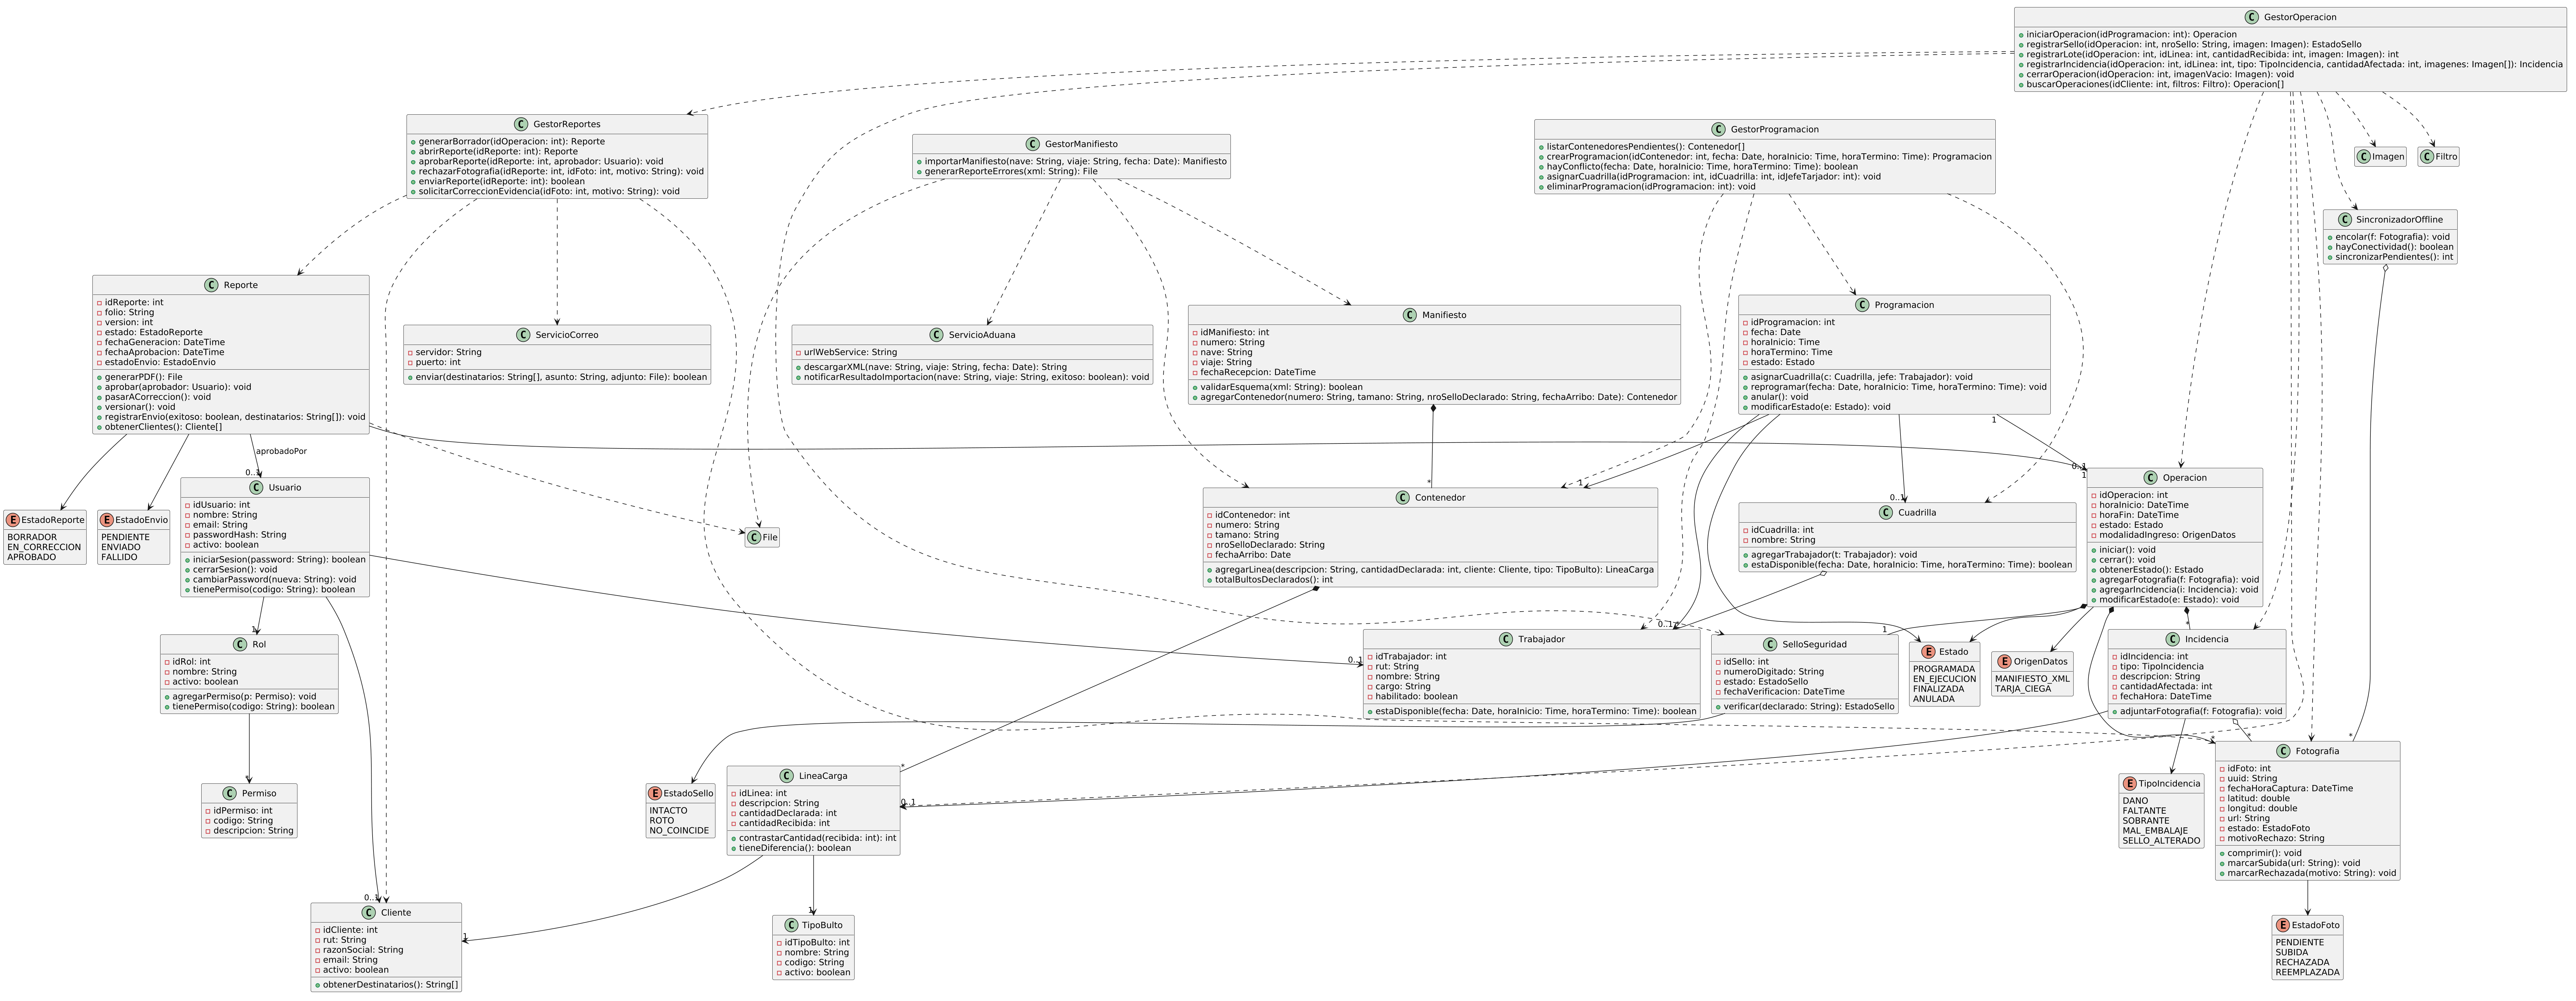
\includegraphics[width=\linewidth]{21-diagrama-clases.png}%
    }{%
        \fbox{\parbox[c][7cm][c]{0.85\linewidth}{\centering
            \textbf{[Diagrama pendiente]}\\[4pt]
            \texttt{Figuras/diagramas/21-diagrama-clases.png}}}%
    }
    \caption[Diagrama de clases]{Diagrama de clases del sistema BeeTracer.}
    \label{fig:clases}
\end{figure}
\vfill
\end{landscape}

\fussy


\chapter{Diccionario de Clases}
\label{cap:diccionario}

Se documenta cada clase del diagrama de diseño indicando su responsabilidad, sus atributos y sus
operaciones principales. La notación de visibilidad sigue el estándar UML: \texttt{-} privado,
\texttt{+} público, \texttt{\#} protegido.

En cada tabla, el bloque \textbf{Atributos} indica nombre, tipo y descripción, y el bloque
\textbf{Operaciones} presenta la firma completa y su descripción.

\section{Paquete «Seguridad y maestros»}
\label{sec:pkg_maestros}

\subsection{Clase \clase{Deposito}}

\textbf{Responsabilidad:} representa al terminal extraportuario, depósito o bodega que opera el
sistema. Es la raíz de la configuración: todos los maestros y operaciones le pertenecen.

{\estilotabla
\begin{longtable}{L{0.26\textwidth} L{0.12\textwidth} L{0.54\textwidth}}
\caption{Clase \clase{Deposito}: atributos y operaciones}\label{tab:cls_deposito}\\
\toprule
\multicolumn{3}{l}{\cellcolor{filacabecera}\textbf{Atributos}} \\
\midrule
\textbf{Nombre} & \textbf{Tipo} & \textbf{Descripción} \\
\midrule
\endfirsthead
\toprule
\textbf{Nombre} & \textbf{Tipo} & \textbf{Descripción} \\
\midrule
\endhead
\clase{idDeposito} & int & Identificador único del depósito. \\
\clase{rut} & String & Identificación tributaria de la organización. \\
\clase{razonSocial} & String & Nombre legal del terminal o bodega. \\
\clase{direccion} & String & Ubicación física del recinto. \\
\clase{zonaHoraria} & String & Zona horaria de operación. Relevante para la
internacionalización. \\
\midrule
\multicolumn{3}{l}{\cellcolor{filacabecera}\textbf{Operaciones}} \\
\midrule
\multicolumn{2}{L{0.40\textwidth}}{\clase{+ obtenerParametros() : Parametro[]}} &
Recupera la parametrización vigente del depósito. \\
\bottomrule
\end{longtable}
}

\subsection{Clase \clase{Usuario}}

\textbf{Responsabilidad:} representa a una persona con acceso al sistema, en web o móvil.
Concentra la autenticación y la resolución de permisos.

{\estilotabla
\begin{longtable}{L{0.26\textwidth} L{0.12\textwidth} L{0.54\textwidth}}
\caption{Clase \clase{Usuario}: atributos y operaciones}\label{tab:cls_usuario}\\
\toprule
\multicolumn{3}{l}{\cellcolor{filacabecera}\textbf{Atributos}} \\
\midrule
\textbf{Nombre} & \textbf{Tipo} & \textbf{Descripción} \\
\midrule
\endfirsthead
\toprule
\textbf{Nombre} & \textbf{Tipo} & \textbf{Descripción} \\
\midrule
\endhead
\clase{idUsuario} & int & Identificador único. \\
\clase{nombre} & String & Nombre completo del usuario. \\
\clase{email} & String & Correo electrónico; actúa como identificador de acceso. \\
\clase{passwordHash} & String & Resumen criptográfico de la contraseña. Nunca se almacena en
claro. \\
\clase{activo} & boolean & Indica si la cuenta está habilitada. \\
\clase{ultimoAcceso} & DateTime & Fecha y hora del último ingreso, para la bitácora. \\
\midrule
\multicolumn{3}{l}{\cellcolor{filacabecera}\textbf{Operaciones}} \\
\midrule
\multicolumn{2}{L{0.40\textwidth}}{\clase{+ autenticar(pass : String) : boolean}} &
Valida las credenciales y establece la sesión (CU-22). \\
\multicolumn{2}{L{0.40\textwidth}}{\clase{+ tienePermiso(codigo : String) : boolean}} &
Resuelve si el usuario puede ejecutar una acción, recorriendo sus roles. \\
\multicolumn{2}{L{0.40\textwidth}}{\clase{+ cambiarPassword(nueva : String) : void}} &
Actualiza la contraseña aplicando la función de resumen. \\
\bottomrule
\end{longtable}
}

\subsection{Clase \clase{Rol}}

\textbf{Responsabilidad:} agrupa un conjunto de permisos bajo un nombre, para asignarlos en bloque.
Permite definir perfiles a medida (administrador, jefe de faena, jefe tarjador, supervisor).

{\estilotabla
\begin{longtable}{L{0.26\textwidth} L{0.12\textwidth} L{0.54\textwidth}}
\caption{Clase \clase{Rol}: atributos y operaciones}\label{tab:cls_rol}\\
\toprule
\multicolumn{3}{l}{\cellcolor{filacabecera}\textbf{Atributos}} \\
\midrule
\textbf{Nombre} & \textbf{Tipo} & \textbf{Descripción} \\
\midrule
\endfirsthead
\toprule
\textbf{Nombre} & \textbf{Tipo} & \textbf{Descripción} \\
\midrule
\endhead
\clase{idRol} & int & Identificador único. \\
\clase{nombre} & String & Denominación del perfil. \\
\clase{descripcion} & String & Alcance del rol. \\
\midrule
\multicolumn{3}{l}{\cellcolor{filacabecera}\textbf{Operaciones}} \\
\midrule
\multicolumn{2}{L{0.40\textwidth}}{\clase{+ agregarPermiso(p : Permiso) : void}} &
Incorpora un permiso al rol. \\
\bottomrule
\end{longtable}
}

\subsection{Clase \clase{Permiso}}

\textbf{Responsabilidad:} representa la autorización atómica para ejecutar una funcionalidad
concreta.

{\estilotabla
\begin{longtable}{L{0.26\textwidth} L{0.12\textwidth} L{0.54\textwidth}}
\caption{Clase \clase{Permiso}: atributos}\label{tab:cls_permiso}\\
\toprule
\textbf{Nombre} & \textbf{Tipo} & \textbf{Descripción} \\
\midrule
\endfirsthead
\toprule
\textbf{Nombre} & \textbf{Tipo} & \textbf{Descripción} \\
\midrule
\endhead
\clase{idPermiso} & int & Identificador único. \\
\clase{codigo} & String & Clave interna de la funcionalidad protegida (p. ej.
\estado{REPORTE\_APROBAR}). \\
\clase{descripcion} & String & Explicación legible del permiso. \\
\bottomrule
\end{longtable}
}

\subsection{Clase \clase{Cliente}}

\textbf{Responsabilidad:} representa a la empresa importadora consignataria de la carga. Es el
destinatario del reporte.

{\estilotabla
\begin{longtable}{L{0.26\textwidth} L{0.12\textwidth} L{0.54\textwidth}}
\caption{Clase \clase{Cliente}: atributos y operaciones}\label{tab:cls_cliente}\\
\toprule
\multicolumn{3}{l}{\cellcolor{filacabecera}\textbf{Atributos}} \\
\midrule
\textbf{Nombre} & \textbf{Tipo} & \textbf{Descripción} \\
\midrule
\endfirsthead
\toprule
\textbf{Nombre} & \textbf{Tipo} & \textbf{Descripción} \\
\midrule
\endhead
\clase{idCliente} & int & Identificador único. \\
\clase{rut} & String & Identificación tributaria del importador. \\
\clase{razonSocial} & String & Nombre legal de la empresa. \\
\clase{emailContacto} & String & Correo principal de contacto. \\
\clase{telefono} & String & Teléfono de contacto. \\
\clase{activo} & boolean & Indica si el cliente está vigente. \\
\midrule
\multicolumn{3}{l}{\cellcolor{filacabecera}\textbf{Operaciones}} \\
\midrule
\multicolumn{2}{L{0.40\textwidth}}{\clase{+ obtenerDestinatarios() : String[]}} &
Devuelve las direcciones de correo a las que debe enviarse el reporte (CU-20). \\
\bottomrule
\end{longtable}
}

\subsection{Clase \clase{Trabajador}}

\textbf{Responsabilidad:} representa al personal operativo del depósito que conforma las
cuadrillas.

{\estilotabla
\begin{longtable}{L{0.26\textwidth} L{0.12\textwidth} L{0.54\textwidth}}
\caption{Clase \clase{Trabajador}: atributos y operaciones}\label{tab:cls_trabajador}\\
\toprule
\multicolumn{3}{l}{\cellcolor{filacabecera}\textbf{Atributos}} \\
\midrule
\textbf{Nombre} & \textbf{Tipo} & \textbf{Descripción} \\
\midrule
\endfirsthead
\toprule
\textbf{Nombre} & \textbf{Tipo} & \textbf{Descripción} \\
\midrule
\endhead
\clase{idTrabajador} & int & Identificador único. \\
\clase{rut} & String & Identificación del trabajador. \\
\clase{nombre} & String & Nombre completo. \\
\clase{cargo} & String & Función que desempeña (p. ej. jefe tarjador, estibador). \\
\clase{habilitado} & boolean & Indica si puede ser asignado a faenas. \\
\midrule
\multicolumn{3}{l}{\cellcolor{filacabecera}\textbf{Operaciones}} \\
\midrule
\multicolumn{2}{L{0.40\textwidth}}{\clase{+ estaDisponible(f : Date, h : Time) : boolean}} &
Verifica que no tenga otra faena asignada en la franja indicada (CU-09). \\
\bottomrule
\end{longtable}
}

\subsection{Clase \clase{Cuadrilla}}

\textbf{Responsabilidad:} agrupa a los cuatro o cinco trabajadores que ejecutan físicamente una
faena de desconsolidado, uno de los cuales opera la aplicación móvil.

{\estilotabla
\begin{longtable}{L{0.26\textwidth} L{0.12\textwidth} L{0.54\textwidth}}
\caption{Clase \clase{Cuadrilla}: atributos y operaciones}\label{tab:cls_cuadrilla}\\
\toprule
\multicolumn{3}{l}{\cellcolor{filacabecera}\textbf{Atributos}} \\
\midrule
\textbf{Nombre} & \textbf{Tipo} & \textbf{Descripción} \\
\midrule
\endfirsthead
\toprule
\textbf{Nombre} & \textbf{Tipo} & \textbf{Descripción} \\
\midrule
\endhead
\clase{idCuadrilla} & int & Identificador único. \\
\clase{nombre} & String & Denominación de la cuadrilla. \\
\clase{turno} & String & Turno de trabajo asociado. \\
\midrule
\multicolumn{3}{l}{\cellcolor{filacabecera}\textbf{Operaciones}} \\
\midrule
\multicolumn{2}{L{0.40\textwidth}}{\clase{+ agregarTrabajador(t : Trabajador) : void}} &
Incorpora un integrante a la cuadrilla. \\
\multicolumn{2}{L{0.40\textwidth}}{\clase{+ obtenerJefeTarjador() : Trabajador}} &
Devuelve al integrante designado como responsable de la aplicación móvil. \\
\multicolumn{2}{L{0.40\textwidth}}{\clase{+ estaDisponible(f : Date, h : Time) : boolean}} &
Verifica la disponibilidad del equipo completo para la franja indicada. \\
\bottomrule
\end{longtable}
}

\subsection{Clase \clase{TipoBulto}}

\textbf{Responsabilidad:} parametriza las unidades con que se registra la carga (caja, pallet,
atado, bobina), permitiendo adaptar el sistema a la operación de cada depósito.

{\estilotabla
\begin{longtable}{L{0.26\textwidth} L{0.12\textwidth} L{0.54\textwidth}}
\caption{Clase \clase{TipoBulto}: atributos}\label{tab:cls_tipobulto}\\
\toprule
\textbf{Nombre} & \textbf{Tipo} & \textbf{Descripción} \\
\midrule
\endfirsthead
\toprule
\textbf{Nombre} & \textbf{Tipo} & \textbf{Descripción} \\
\midrule
\endhead
\clase{idTipoBulto} & int & Identificador único. \\
\clase{nombre} & String & Denominación del tipo de bulto. \\
\clase{descripcion} & String & Detalle del tipo. \\
\clase{unidadMedida} & String & Unidad en que se cuantifica. \\
\bottomrule
\end{longtable}
}

\section{Paquete «Información de carga»}
\label{sec:pkg_carga}

\subsection{Clase \clase{Manifiesto}}

\textbf{Responsabilidad:} representa el documento oficial que declara la totalidad de la carga que
transporta una nave. Es la fuente de verdad de referencia del sistema.

{\estilotabla
\begin{longtable}{L{0.26\textwidth} L{0.12\textwidth} L{0.54\textwidth}}
\caption{Clase \clase{Manifiesto}: atributos y operaciones}\label{tab:cls_manifiesto}\\
\toprule
\multicolumn{3}{l}{\cellcolor{filacabecera}\textbf{Atributos}} \\
\midrule
\textbf{Nombre} & \textbf{Tipo} & \textbf{Descripción} \\
\midrule
\endfirsthead
\toprule
\textbf{Nombre} & \textbf{Tipo} & \textbf{Descripción} \\
\midrule
\endhead
\clase{idManifiesto} & int & Identificador único. \\
\clase{numeroManifiesto} & String & Folio oficial asignado por Aduanas. \\
\clase{nave} & String & Nombre de la nave que transporta la carga. \\
\clase{viaje} & String & Identificador del viaje. \\
\clase{fechaRecepcion} & DateTime & Momento en que el sistema descargó el documento. \\
\clase{origenDatos} & OrigenDatos & Vía por la que ingresó la información (XML, API o tarja
ciega). \\
\midrule
\multicolumn{3}{l}{\cellcolor{filacabecera}\textbf{Operaciones}} \\
\midrule
\multicolumn{2}{L{0.40\textwidth}}{\clase{+ cargarDesdeXML(xml : String) : boolean}} &
Interpreta el documento XML y construye la jerarquía de contenedores y líneas de carga
(CU-05). \\
\multicolumn{2}{L{0.40\textwidth}}{\clase{+ validarEsquema() : boolean}} &
Verifica que el XML cumpla el estándar esperado antes de procesarlo. \\
\multicolumn{2}{L{0.40\textwidth}}{\clase{+ agregarContenedor(c : Contenedor) : void}} &
Asocia un contenedor al manifiesto. \\
\bottomrule
\end{longtable}
}

\subsection{Clase \clase{Contenedor}}

\textbf{Responsabilidad:} representa la unidad física de transporte que será desconsolidada.

{\estilotabla
\begin{longtable}{L{0.26\textwidth} L{0.12\textwidth} L{0.54\textwidth}}
\caption{Clase \clase{Contenedor}: atributos y operaciones}\label{tab:cls_contenedor}\\
\toprule
\multicolumn{3}{l}{\cellcolor{filacabecera}\textbf{Atributos}} \\
\midrule
\textbf{Nombre} & \textbf{Tipo} & \textbf{Descripción} \\
\midrule
\endfirsthead
\toprule
\textbf{Nombre} & \textbf{Tipo} & \textbf{Descripción} \\
\midrule
\endhead
\clase{idContenedor} & int & Identificador único interno. \\
\clase{sigla} & String & Prefijo del propietario del contenedor (estándar ISO). \\
\clase{numero} & String & Número identificador del contenedor. \\
\clase{tipo} & String & Tipo de contenedor (\este{dry}, \este{reefer}, \este{open top}). \\
\clase{tamano} & String & Dimensión (20', 40', 40'HC). \\
\clase{nroSelloDeclarado} & String & Número de sello de seguridad según el manifiesto. Se contrasta
en terreno. \\
\clase{fechaArribo} & Date & Fecha estimada o efectiva de llegada. \\
\midrule
\multicolumn{3}{l}{\cellcolor{filacabecera}\textbf{Operaciones}} \\
\midrule
\multicolumn{2}{L{0.40\textwidth}}{\clase{+ agregarLinea(l : LineaCarga) : void}} &
Asocia una línea de carga al contenedor. \\
\multicolumn{2}{L{0.40\textwidth}}{\clase{+ totalBultosDeclarados() : int}} &
Suma las cantidades declaradas de todas sus líneas. \\
\bottomrule
\end{longtable}
}

\subsection{Clase \clase{LineaCarga}}

\textbf{Responsabilidad:} representa el lote de mercancía consignado a un cliente específico dentro
de un contenedor. \textbf{Es la clase donde se materializa el contraste entre lo declarado y lo
recibido.}

{\estilotabla
\begin{longtable}{L{0.26\textwidth} L{0.12\textwidth} L{0.54\textwidth}}
\caption{Clase \clase{LineaCarga}: atributos y operaciones}\label{tab:cls_lineacarga}\\
\toprule
\multicolumn{3}{l}{\cellcolor{filacabecera}\textbf{Atributos}} \\
\midrule
\textbf{Nombre} & \textbf{Tipo} & \textbf{Descripción} \\
\midrule
\endfirsthead
\toprule
\textbf{Nombre} & \textbf{Tipo} & \textbf{Descripción} \\
\midrule
\endhead
\clase{idLinea} & int & Identificador único. \\
\clase{blConocimiento} & String & Número del conocimiento de embarque (\este{Bill of Lading}). \\
\clase{descripcion} & String & Descripción de la mercancía. \\
\clase{marcas} & String & Marcas y contramarcas impresas en los bultos. \\
\clase{cantidadDeclarada} & int & Número de bultos según el manifiesto. Nulo en modalidad tarja
ciega. \\
\clase{cantidadRecibida} & int & Número de bultos efectivamente contados en terreno. \\
\clase{pesoKg} & decimal & Peso declarado del lote. \\
\midrule
\multicolumn{3}{l}{\cellcolor{filacabecera}\textbf{Operaciones}} \\
\midrule
\multicolumn{2}{L{0.40\textwidth}}{\clase{+ contrastarCantidad(recibida : int) : int}} &
Registra la cantidad recibida y devuelve la diferencia respecto de la declarada. \\
\multicolumn{2}{L{0.40\textwidth}}{\clase{+ tieneDiferencia() : boolean}} &
Indica si existe faltante o sobrante, disparando la creación de una incidencia. \\
\bottomrule
\end{longtable}
}

\subsection{Enumeración \clase{OrigenDatos}}

\clase{MANIFIESTO\_XML} $\cdot$ \clase{INTEGRACION\_API} $\cdot$ \clase{TARJA\_CIEGA}: identifica la
vía por la que ingresó la información de la carga. Condiciona si el contraste de cantidades es
aplicable.

\section{Paquete «Operación en terreno»}
\label{sec:pkg_terreno}

\subsection{Clase \clase{Faena}}

\textbf{Responsabilidad: clase central del modelo.} Representa la operación programada de
desconsolidado de un contenedor: su planificación, ejecución y cierre. Actúa como agregado raíz del
expediente probatorio.

{\estilotabla
\begin{longtable}{L{0.26\textwidth} L{0.12\textwidth} L{0.54\textwidth}}
\caption{Clase \clase{Faena}: atributos y operaciones}\label{tab:cls_faena}\\
\toprule
\multicolumn{3}{l}{\cellcolor{filacabecera}\textbf{Atributos}} \\
\midrule
\textbf{Nombre} & \textbf{Tipo} & \textbf{Descripción} \\
\midrule
\endfirsthead
\toprule
\textbf{Nombre} & \textbf{Tipo} & \textbf{Descripción} \\
\midrule
\endhead
\clase{idFaena} & int & Identificador único. \\
\clase{folio} & String & Número de faena visible para el usuario y en el reporte. \\
\clase{fechaProgramada} & Date & Día en que se ejecutará el desconsolidado. \\
\clase{horaInicio} & Time & Inicio de la franja horaria asignada. \\
\clase{horaTermino} & Time & Término de la franja horaria asignada. \\
\clase{estado} & EstadoFaena & Situación actual de la faena. \\
\clase{modalidadIngreso} & OrigenDatos & Vía por la que se obtuvo la información de la carga. \\
\midrule
\multicolumn{3}{l}{\cellcolor{filacabecera}\textbf{Operaciones}} \\
\midrule
\multicolumn{2}{L{0.40\textwidth}}{\clase{+ programar(f : Date, hi : Time, ht : Time) : void}} &
Fija fecha y franja horaria (CU-08). \\
\multicolumn{2}{L{0.40\textwidth}}{\clase{+ asignarCuadrilla(c : Cuadrilla,
jt : Trabajador) : void}} &
Asocia el equipo de trabajo y designa al responsable de la aplicación móvil (CU-09). \\
\multicolumn{2}{L{0.40\textwidth}}{\clase{+ iniciar() : void}} &
Marca el comienzo efectivo de la faena en terreno. \\
\multicolumn{2}{L{0.40\textwidth}}{\clase{+ registrarEtapa(tipo : TipoEtapa) : EtapaFaena}} &
Abre una nueva etapa del proceso. \\
\multicolumn{2}{L{0.40\textwidth}}{\clase{+ cerrar() : void}} &
Valida la completitud de la evidencia, finaliza la faena y dispara la generación del reporte
(CU-14, CU-17). \\
\multicolumn{2}{L{0.40\textwidth}}{\clase{+ cambiarEstado(e : EstadoFaena) : void}} &
Transiciona el estado respetando las reglas de negocio. \\
\bottomrule
\end{longtable}
}

\subsection{Clase \clase{EtapaFaena}}

\textbf{Responsabilidad:} representa cada uno de los momentos críticos del proceso en los que el
sistema exige evidencia. Impone el orden del flujo en terreno.

{\estilotabla
\begin{longtable}{L{0.26\textwidth} L{0.12\textwidth} L{0.54\textwidth}}
\caption{Clase \clase{EtapaFaena}: atributos y operaciones}\label{tab:cls_etapafaena}\\
\toprule
\multicolumn{3}{l}{\cellcolor{filacabecera}\textbf{Atributos}} \\
\midrule
\textbf{Nombre} & \textbf{Tipo} & \textbf{Descripción} \\
\midrule
\endfirsthead
\toprule
\textbf{Nombre} & \textbf{Tipo} & \textbf{Descripción} \\
\midrule
\endhead
\clase{idEtapa} & int & Identificador único. \\
\clase{tipo} & TipoEtapa & Momento del proceso que representa. \\
\clase{fechaHoraInicio} & DateTime & Marca de tiempo de apertura de la etapa. \\
\clase{fechaHoraFin} & DateTime & Marca de tiempo de cierre de la etapa. \\
\clase{observacion} & String & Comentario libre del operario. \\
\midrule
\multicolumn{3}{l}{\cellcolor{filacabecera}\textbf{Operaciones}} \\
\midrule
\multicolumn{2}{L{0.40\textwidth}}{\clase{+ agregarEvidencia(f : Fotografia) : void}} &
Asocia una fotografía a la etapa. \\
\multicolumn{2}{L{0.40\textwidth}}{\clase{+ estaCompleta() : boolean}} &
Verifica que la etapa cuente con la evidencia obligatoria antes de permitir el avance. \\
\bottomrule
\end{longtable}
}

\subsection{Clase \clase{SelloSeguridad}}

\textbf{Responsabilidad:} registra la verificación del sello del contenedor, uno de los elementos
de mayor valor probatorio de toda la faena.

{\estilotabla
\begin{longtable}{L{0.26\textwidth} L{0.12\textwidth} L{0.54\textwidth}}
\caption{Clase \clase{SelloSeguridad}: atributos y operaciones}\label{tab:cls_sello}\\
\toprule
\multicolumn{3}{l}{\cellcolor{filacabecera}\textbf{Atributos}} \\
\midrule
\textbf{Nombre} & \textbf{Tipo} & \textbf{Descripción} \\
\midrule
\endfirsthead
\toprule
\textbf{Nombre} & \textbf{Tipo} & \textbf{Descripción} \\
\midrule
\endhead
\clase{idSello} & int & Identificador único. \\
\clase{numeroDigitado} & String & Número que el operario leyó y digitó en terreno. \\
\clase{estado} & EstadoSello & Resultado de la verificación. \\
\clase{fechaVerificacion} & DateTime & Momento de la verificación. \\
\midrule
\multicolumn{3}{l}{\cellcolor{filacabecera}\textbf{Operaciones}} \\
\midrule
\multicolumn{2}{L{0.40\textwidth}}{\clase{+ verificarContraDeclarado(dec : String) :
EstadoSello}} &
Compara el número digitado contra el declarado en el manifiesto y determina si el sello está
intacto, roto o no coincide. \\
\bottomrule
\end{longtable}
}

\subsection{Clase \clase{Fotografia}}

\textbf{Responsabilidad: unidad de evidencia del sistema.} Encapsula la imagen capturada en terreno
junto con los metadatos que le otorgan valor probatorio, y gestiona su ciclo de compresión y
subida.

{\estilotabla
\begin{longtable}{L{0.26\textwidth} L{0.12\textwidth} L{0.54\textwidth}}
\caption{Clase \clase{Fotografia}: atributos y operaciones}\label{tab:cls_fotografia}\\
\toprule
\multicolumn{3}{l}{\cellcolor{filacabecera}\textbf{Atributos}} \\
\midrule
\textbf{Nombre} & \textbf{Tipo} & \textbf{Descripción} \\
\midrule
\endfirsthead
\toprule
\textbf{Nombre} & \textbf{Tipo} & \textbf{Descripción} \\
\midrule
\endhead
\clase{idFoto} & int & Identificador único. \\
\clase{uuid} & String & Identificador universal generado en el dispositivo, previo a la subida. \\
\clase{nombreArchivo} & String & Nombre del archivo de imagen. \\
\clase{url} & String & Dirección en el repositorio en la nube, una vez subida. \\
\clase{fechaHoraCaptura} & DateTime & Momento exacto de la captura. Elemento probatorio clave. \\
\clase{latitud} & decimal & Latitud de la captura. \\
\clase{longitud} & decimal & Longitud de la captura. \\
\clase{tamanoBytes} & long & Peso del archivo tras la compresión. \\
\clase{hash} & String & Resumen criptográfico de la imagen, para verificar su integridad. \\
\clase{estado} & EstadoFoto & Situación de la fotografía en su ciclo de vida. \\
\clase{motivoRechazo} & String & Razón indicada por el Supervisor al rechazarla (CU-19). \\
\midrule
\multicolumn{3}{l}{\cellcolor{filacabecera}\textbf{Operaciones}} \\
\midrule
\multicolumn{2}{L{0.40\textwidth}}{\clase{+ comprimir() : void}} &
Reduce el peso de la imagen en el dispositivo manteniendo legibilidad suficiente como
evidencia. \\
\multicolumn{2}{L{0.40\textwidth}}{\clase{+ subir() : boolean}} &
Transfiere la imagen al repositorio en la nube. \\
\multicolumn{2}{L{0.40\textwidth}}{\clase{+ marcarSubida(url : String) : void}} &
Confirma la subida y registra la dirección definitiva. \\
\multicolumn{2}{L{0.40\textwidth}}{\clase{+ marcarRechazada(motivo : String) : void}} &
Invalida la fotografía y registra el motivo, solicitando recaptura. \\
\bottomrule
\end{longtable}
}

\subsection{Clase \clase{Incidencia}}

\textbf{Responsabilidad:} documenta toda anomalía detectada en la carga. Es la información que
activa los seguros y delimita las responsabilidades entre naviera, terminal e importador.

{\estilotabla
\begin{longtable}{L{0.26\textwidth} L{0.12\textwidth} L{0.54\textwidth}}
\caption{Clase \clase{Incidencia}: atributos y operaciones}\label{tab:cls_incidencia}\\
\toprule
\multicolumn{3}{l}{\cellcolor{filacabecera}\textbf{Atributos}} \\
\midrule
\textbf{Nombre} & \textbf{Tipo} & \textbf{Descripción} \\
\midrule
\endfirsthead
\toprule
\textbf{Nombre} & \textbf{Tipo} & \textbf{Descripción} \\
\midrule
\endhead
\clase{idIncidencia} & int & Identificador único. \\
\clase{tipo} & TipoIncidencia & Naturaleza de la anomalía. \\
\clase{descripcion} & String & Relato del operario sobre lo observado. \\
\clase{cantidadAfectada} & int & Número de bultos comprometidos. \\
\clase{gravedad} & String & Clasificación de severidad del hecho. \\
\clase{fechaHora} & DateTime & Momento de la detección. \\
\midrule
\multicolumn{3}{l}{\cellcolor{filacabecera}\textbf{Operaciones}} \\
\midrule
\multicolumn{2}{L{0.40\textwidth}}{\clase{+ adjuntarFotografia(f : Fotografia) : void}} &
Asocia evidencia exclusiva a la incidencia. Obligatorio (RI-2). \\
\bottomrule
\end{longtable}
}

\subsection{Enumeraciones del paquete}

{\estilotabla
\begin{longtable}{L{0.18\textwidth} L{0.40\textwidth} L{0.36\textwidth}}

\caption{Enumeraciones del paquete «Operación en terreno»}
\label{tab:enum_terreno}
\\

\toprule
\textbf{Enumeración} & \textbf{Valores} & \textbf{Uso} \\
\midrule
\endfirsthead

\toprule
\textbf{Enumeración} & \textbf{Valores} & \textbf{Uso} \\
\midrule
\endhead

\clase{EstadoFaena} &
\estado{PROGRAMADA} $\cdot$ \estado{EN\_EJECUCION} $\cdot$ \estado{FINALIZADA} $\cdot$
\estado{ANULADA} &
Ciclo de vida de la operación. \\
\midrule

\clase{TipoEtapa} &
\estado{APERTURA} $\cdot$ \estado{SEPARACION} $\cdot$ \estado{INCIDENCIA} $\cdot$
\estado{CIERRE} &
Momentos críticos que exigen evidencia. \\
\midrule

\clase{EstadoSello} &
\estado{INTACTO} $\cdot$ \estado{ROTO} $\cdot$ \estado{NO\_COINCIDE} &
Resultado de la verificación del sello. \\
\midrule

\clase{EstadoFoto} &
\estado{PENDIENTE} $\cdot$ \estado{SUBIDA} $\cdot$ \estado{RECHAZADA} $\cdot$
\estado{REEMPLAZADA} &
Ciclo de vida de la evidencia, incluyendo el modo offline y la recaptura. \\
\midrule

\clase{TipoIncidencia} &
\estado{DANO} $\cdot$ \estado{FALTANTE} $\cdot$ \estado{SOBRANTE} $\cdot$
\estado{MAL\_EMBALADO} &
Clasificación de las anomalías. \\

\bottomrule

\end{longtable}
}

\section{Paquete «Reportes y publicación»}
\label{sec:pkg_reportes}

\subsection{Clase \clase{Reporte}}

\textbf{Responsabilidad:} consolida el expediente completo de una faena en un documento PDF
verificable y gestiona su ciclo de revisión, aprobación y publicación.

{\estilotabla
\begin{longtable}{L{0.26\textwidth} L{0.12\textwidth} L{0.54\textwidth}}
\caption{Clase \clase{Reporte}: atributos y operaciones}\label{tab:cls_reporte}\\
\toprule
\multicolumn{3}{l}{\cellcolor{filacabecera}\textbf{Atributos}} \\
\midrule
\textbf{Nombre} & \textbf{Tipo} & \textbf{Descripción} \\
\midrule
\endfirsthead
\toprule
\textbf{Nombre} & \textbf{Tipo} & \textbf{Descripción} \\
\midrule
\endhead
\clase{idReporte} & int & Identificador único. \\
\clase{folio} & String & Número visible del reporte. \\
\clase{version} & int & Número de versión, que se incrementa tras cada ciclo de recaptura. \\
\clase{fechaGeneracion} & DateTime & Momento de generación del borrador. \\
\clase{fechaAprobacion} & DateTime & Momento de la aprobación por el Supervisor. \\
\clase{estado} & EstadoReporte & Situación del reporte en su flujo. \\
\clase{urlPdf} & String & Ubicación del archivo PDF generado. \\
\midrule
\multicolumn{3}{l}{\cellcolor{filacabecera}\textbf{Operaciones}} \\
\midrule
\multicolumn{2}{L{0.40\textwidth}}{\clase{+ generarPDF() : Archivo}} &
Solicita la composición del documento a partir de los datos y fotografías de la faena (CU-17). \\
\multicolumn{2}{L{0.40\textwidth}}{\clase{+ versionar() : void}} &
Incrementa la versión preservando el historial tras una corrección. \\
\multicolumn{2}{L{0.40\textwidth}}{\clase{+ aprobar(s : Usuario, fh : DateTime) : void}} &
Registra quién aprobó el reporte y cuándo, habilitando su envío (CU-18). \\
\multicolumn{2}{L{0.40\textwidth}}{\clase{+ obtenerDestinatarios() : String[]}} &
Reúne los correos de todos los clientes involucrados en la faena. \\
\multicolumn{2}{L{0.40\textwidth}}{\clase{+ registrarEnvio(e : EnvioReporte) : void}} &
Deja constancia del despacho del documento. \\
\bottomrule
\end{longtable}
}

\subsection{Clase \clase{EnvioReporte}}

\textbf{Responsabilidad:} registra cada intento de despacho del reporte, exitoso o fallido, como
parte del expediente probatorio.

{\estilotabla
\begin{longtable}{L{0.26\textwidth} L{0.12\textwidth} L{0.54\textwidth}}
\caption{Clase \clase{EnvioReporte}: atributos y operaciones}\label{tab:cls_envioreporte}\\
\toprule
\multicolumn{3}{l}{\cellcolor{filacabecera}\textbf{Atributos}} \\
\midrule
\textbf{Nombre} & \textbf{Tipo} & \textbf{Descripción} \\
\midrule
\endfirsthead
\toprule
\textbf{Nombre} & \textbf{Tipo} & \textbf{Descripción} \\
\midrule
\endhead
\clase{idEnvio} & int & Identificador único. \\
\clase{fechaHoraEnvio} & DateTime & Momento del intento de envío. \\
\clase{destinatarios} & String & Direcciones a las que se despachó el documento. \\
\clase{estadoEnvio} & String & Resultado del intento (\estado{ENVIADO} / \estado{FALLIDO}). \\
\clase{mensajeError} & String & Detalle del fallo, cuando corresponde. \\
\clase{intentos} & int & Número de reintentos acumulados. \\
\midrule
\multicolumn{3}{l}{\cellcolor{filacabecera}\textbf{Operaciones}} \\
\midrule
\multicolumn{2}{L{0.40\textwidth}}{\clase{+ reintentar() : boolean}} &
Vuelve a despachar el documento tras un fallo. \\
\bottomrule
\end{longtable}
}

\subsection{Enumeración \clase{EstadoReporte}}

\estado{BORRADOR} $\cdot$ \estado{EN\_CORRECCION} $\cdot$ \estado{APROBADO} $\cdot$
\estado{ENVIADO}: refleja el flujo de control de calidad descrito en CU-18 y CU-19.

\section{Paquete «Controladores y servicios»}
\label{sec:pkg_controladores}

{\estilotabla
\begin{longtable}{L{0.17\textwidth} L{0.10\textwidth} L{0.37\textwidth} L{0.28\textwidth}}

\caption{Controladores, interfaces y servicios del diseño}
\label{tab:controladores}
\\

\toprule
\textbf{Clase} & \textbf{Estereo\-tipo} & \textbf{Responsabilidad} &
\textbf{Operaciones principales} \\
\midrule
\endfirsthead

\toprule
\textbf{Clase} & \textbf{Estereo\-tipo} & \textbf{Responsabilidad} &
\textbf{Operaciones principales} \\
\midrule
\endhead

\clase{Gestor\-Manifiesto} & \ster{control} &
Coordina la ingesta de información de carga por sus tres vías. &
\clase{importarManifiesto()}, \clase{recibirDesdeAPI()}, \clase{declararTarjaCiega()} \\
\midrule

\clase{Gestor\-Programacion} & \ster{control} &
Coordina la planificación de faenas y la asignación de recursos. &
\clase{listarContenedoresPendientes()}, \clase{programarFaena()}, \clase{asignarCuadrilla()},
\clase{validarDisponibilidadHorario()} \\
\midrule

\clase{GestorFaena} & \ster{control} &
Coordina la ejecución de la faena en terreno. Es el controlador con mayor tráfico de mensajes del
sistema. &
\clase{iniciarFaena()}, \clase{verificarSello()}, \clase{registrarLote()},
\clase{registrarIncidencia()}, \clase{registrarEvidencia()}, \clase{cerrarFaena()} \\
\midrule

\clase{Gestor\-Reportes} & \ster{control} &
Coordina la generación, revisión, aprobación y publicación del reporte. &
\clase{generarBorrador()}, \clase{rechazarFotografia()}, \clase{aprobarReporte()},
\clase{enviarReporte()} \\
\midrule

\clase{Sincronizador\-Offline} & \ster{control} &
Desacopla la captura de evidencia de su transmisión. Mantiene la cola de pendientes y gestiona los
reintentos. Es el único objeto que conoce el repositorio externo. &
\clase{encolarSubida()}, \clase{hayConectividad()}, \clase{sincronizarPendientes()},
\clase{persistirLocal()} \\
\midrule

\clase{IServicio\-Aduana} & \ster{interface} &
Abstrae la comunicación con la aduana, permitiendo la internacionalización sin modificar el resto
del sistema. &
\clase{descargarXML()} \\
\midrule

\clase{Servicio\-AduanaWS} & --- &
Implementación concreta del \este{web service} del Servicio Nacional de Aduanas de Chile. &
\clase{descargarXML()} \\
\midrule

\clase{IPasarela\-Correo} & \ster{interface} &
Abstrae el despacho de correo electrónico. &
\clase{enviar()} \\
\midrule

\clase{Servicio\-CorreoSMTP} & --- &
Implementación concreta sobre protocolo SMTP. &
\clase{enviar()} \\
\midrule

\clase{GeneradorPDF} & \ster{service} &
Compone el documento PDF a partir de datos y fotografías, destacando las incidencias. Corresponde
al rol que cumplía JasperReports en la versión original del sistema. &
\clase{armarReporte()}, \clase{destacarIncidencias()} \\
\midrule

\clase{Repositorio\-Fotos} & \ster{service} &
Almacenamiento externo de las imágenes capturadas en terreno. &
\clase{subir()}, \clase{obtenerURL()}, \clase{eliminar()} \\

\bottomrule

\end{longtable}
}


\chapter{Conclusiones}
\label{cap:conclusiones}

\begin{pendiente}[Por completar / personalizar]
Las conclusiones que siguen son una propuesta redactada a partir del trabajo efectivamente
realizado. Conviene ajustarlas a la experiencia concreta del equipo y agregar el aprendizaje
personal de cada integrante, que es lo que el profesor suele valorar en esta sección.
\end{pendiente}

\textbf{Sobre el modelado del sistema.} El ejercicio confirma que es posible reconstruir la
arquitectura funcional y estructural de un sistema en producción \textbf{sin acceso a su código
fuente}, partiendo de la descripción del proceso de negocio y de la observación de su
comportamiento externo. El modelo UML resultante no pretende ser idéntico a la implementación real
de BeeTracer, pero sí constituye un \textbf{plano coherente y completo} que explica todo el
comportamiento observado y que serviría de base para construir o extender un sistema equivalente.

\textbf{Sobre el traslado del modelo estructurado al orientado a objetos.} El paso del Informe 1
---con sus diagramas de flujo de datos y su modelo entidad-relación--- a este informe evidenció una
diferencia importante de enfoque. Mientras el modelo estructurado describe \textbf{qué
transformaciones sufre la información}, el modelo orientado a objetos obliga a decidir
\textbf{quién es responsable de cada comportamiento}. Esa decisión no es trivial y en varios puntos
del diseño fue necesario resolverla explícitamente, como al separar \clase{SincronizadorOffline}
del \clase{GestorFaena} o al escoger entre asociar las fotografías a la etapa o a la incidencia.

\textbf{Sobre el dominio.} El estudio del caso reveló que el valor central de BeeTracer \textbf{no
es tecnológico sino probatorio}. El sistema no compite por procesar más rápido ni por almacenar más
datos: compite por producir, en el momento exacto en que la carga cambia de custodia, una evidencia
fechada, geolocalizada y difícil de refutar. Toda su arquitectura se subordina a ese objetivo: por
eso la aplicación \textbf{bloquea el avance} si falta una fotografía, por eso sube las imágenes una
por una en lugar de esperar al final, y por eso existe una etapa de revisión humana antes de que el
reporte llegue al cliente.

\textbf{Sobre las restricciones del entorno como motor del diseño.} Uno de los aprendizajes más
claros del caso es que \textbf{las decisiones de arquitectura más determinantes no nacieron de
requisitos funcionales, sino de restricciones físicas del entorno}. El bloqueo de la señal Wi-Fi
por los contenedores metálicos explica el envío incremental, la compresión en dispositivo y el modo
offline completo. El hecho de que el operario trabaje con guantes y bajo presión de tiempo explica
el flujo guiado paso a paso. La sensibilidad comercial de la evidencia explica la eliminación de la
visualización en vivo por parte del cliente. Un modelo construido solo desde los requisitos
declarados habría omitido lo más característico del sistema.

\textbf{Sobre las limitaciones del trabajo.} El modelo presentado tiene un grado de inferencia
significativo. Las clases, atributos y multiplicidades son una propuesta coherente, pero no
verificada contra la implementación real. Los módulos complementarios ---visor 3D y aplicación de
avisos de transporte--- quedaron fuera del alcance por falta de información. Asimismo, no fue
posible validar el modelo con el equipo desarrollador, lo que habría permitido contrastar las
hipótesis de diseño.

\textbf{Proyección.} El modelo obtenido habilita al menos tres líneas de trabajo futuro:
\textbf{(i)} la incorporación de grabación de video del desconsolidado, funcionalidad que el propio
equipo de BeeTracer evalúa y que el modelo admitiría generalizando \clase{Fotografia} hacia una
clase \clase{Evidencia}; \textbf{(ii)} la integración del visor 3D de patios, añadiendo coordenadas
de ubicación a \clase{Contenedor}; y \textbf{(iii)} la explotación analítica del historial de
incidencias por cliente y por naviera, hoy registrado pero no aprovechado como indicador de
gestión.

\begin{pendiente}
Agregar aquí las conclusiones personales del equipo: dificultades encontradas durante el modelado,
decisiones que se discutieron y cómo se resolvieron, y aprendizaje obtenido de la asignatura.
\end{pendiente}


% =========================================================
% REFERENCIAS BIBLIOGRÁFICAS
% =========================================================

\clearpage
\chapter{Referencias bibliográficas}
\label{cap:referencias}

\nocite{*}
\printbibliography[heading=none]

\end{document}
